% Fichier genere par build.py -- ne pas editer a la main
% =====================================================================
%  Reseaux de neurones recurrents (RNN) -- 20 h -- Master 1 SDIA
%  Preambule commun aux 6 chapitres
%  Moteur : XeLaTeX (Tectonic) -- compilation : voir build.py
% =====================================================================
\documentclass[10pt,aspectratio=169]{beamer}

\usepackage{fontspec}
\usepackage{polyglossia}
\setdefaultlanguage{french}
\usepackage{amsmath,amssymb,mathtools}
\usepackage{unicode-math}
\usepackage{booktabs}
\usepackage{array}
\usepackage{colortbl}
\usepackage{xcolor}
\usepackage{tikz}
\usetikzlibrary{arrows.meta,positioning,calc,shapes.geometric,fit,backgrounds,patterns}
\usepackage{pgfplots}
\pgfplotsset{compat=1.18}
\usepgfplotslibrary{fillbetween}
\usepackage{graphicx}
\usepackage{listings}
\usepackage[most]{tcolorbox}
\tcbuselibrary{skins,breakable}
\usepackage{fontawesome5}
\usepackage{multicol}
\usepackage{multirow}
\usepackage{animate}

% ---------------------------------------------------------------- theme
\usetheme{default}
\usecolortheme{default}
\setbeamertemplate{navigation symbols}{}

\definecolor{byDeep}   {HTML}{10243E}
\definecolor{byBlue}   {HTML}{1F6FEB}
\definecolor{byCyan}   {HTML}{12A594}
\definecolor{byOrange} {HTML}{D97706}
\definecolor{byRed}    {HTML}{C0392B}
\definecolor{byGreen}  {HTML}{1E8449}
\definecolor{byPurple} {HTML}{6C5CE7}
\definecolor{byGrey}   {HTML}{5B6470}
\definecolor{byLight}  {HTML}{F4F6F8}

\setbeamercolor{frametitle}{bg=byDeep,fg=white}
\setbeamercolor{structure}{fg=byBlue}
\setbeamercolor{normal text}{fg=byDeep}
\setbeamercolor{alerted text}{fg=byRed}
\setbeamercolor{title}{fg=white}
\setbeamercolor{subtitle}{fg=white}
\setbeamercolor{author}{fg=white}
\setbeamercolor{date}{fg=white}
\setbeamercolor{item}{fg=byBlue}
\setbeamercolor{section in toc}{fg=byDeep}
\setbeamercolor{block title}{bg=byBlue!12,fg=byDeep}
\setbeamercolor{block body}{bg=byBlue!5}

\setbeamerfont{frametitle}{size=\large,series=\bfseries}
\setbeamerfont{title}{size=\LARGE,series=\bfseries}
\setbeamerfont{block title}{series=\bfseries}

% gain de place vertical : le titre de frame est suivi d'un espace negatif
% (les supports sont denses ; cela evite que le dernier encadre morde sur le pied de page)
\addtobeamertemplate{frametitle}{}{\vspace*{-4.0mm}}
\setlength{\abovedisplayskip}{3pt}
\setlength{\belowdisplayskip}{3pt}
\setlength{\abovedisplayshortskip}{2pt}
\setlength{\belowdisplayshortskip}{2pt}

\setbeamertemplate{itemize item}{\small\raise0.2ex\hbox{\textcolor{byBlue}{$\blacktriangleright$}}}
\setbeamertemplate{itemize subitem}{\tiny\raise0.35ex\hbox{\textcolor{byCyan}{$\bullet$}}}
\setlength{\tabcolsep}{3pt}   % tableaux plus etroits (les slides sont denses)
% listes plus compactes : les supports sont denses et le pied de page mange de la place
\setbeamertemplate{itemize/enumerate body begin}{\vspace*{-2.0mm}}
\setbeamertemplate{itemize/enumerate subbody begin}{\vspace*{-0.6mm}}
\setbeamertemplate{enumerate item}{\textcolor{byBlue}{\bfseries\insertenumlabel.}}
\setbeamertemplate{caption}[numbered]

% footer : chapitre | slide n/N
\setbeamertemplate{footline}{%
  % Beamer reserve la hauteur de cette boite comme zone interdite : le vskip
  % ci-dessous cale la zone de texte exactement au-dessus de la barre visible.
  \vskip 10mm%
  \leavevmode%
  \hbox{%
    \begin{beamercolorbox}[wd=.42\paperwidth,ht=1.9ex,dp=0.8ex,leftskip=.3cm]{author in head/foot}%
      \usebeamerfont{author in head/foot}\color{white}\scriptsize Par Dr. Noulapeu Ngaffo Armielle
    \end{beamercolorbox}%
    \begin{beamercolorbox}[wd=.42\paperwidth,ht=1.9ex,dp=0.8ex,center]{title in head/foot}%
      \usebeamerfont{title in head/foot}\color{white}\scriptsize\insertsectionhead
    \end{beamercolorbox}%
    \begin{beamercolorbox}[wd=.16\paperwidth,ht=1.9ex,dp=0.8ex,rightskip=.3cm]{date in head/foot}%
      \usebeamerfont{date in head/foot}\color{white}\scriptsize\insertframenumber\,/\,\inserttotalframenumber
    \end{beamercolorbox}}%
  \vskip0pt%
}
\setbeamercolor{author in head/foot}{bg=byDeep}
\setbeamercolor{title in head/foot}{bg=byDeep!88}
\setbeamercolor{date in head/foot}{bg=byDeep!76}

\setbeamertemplate{title page}{%
  \begin{tikzpicture}[remember picture,overlay]
    \fill[byDeep] (current page.north west) rectangle (current page.south east);
    \fill[byBlue,opacity=.30] (current page.north east) ++(-3.2,-1.1) circle (5.4cm);
    \fill[byCyan,opacity=.18] (current page.south west) ++(2.2,1.0) circle (4.2cm);
  \end{tikzpicture}
  \vspace{1.1cm}
  \begin{center}
    {\usebeamerfont{title}\usebeamercolor[fg]{title}\inserttitle\par}
    \vspace{.25cm}
    {\large\color{byCyan}\insertsubtitle\par}
    \vspace{.7cm}
    {\color{white}\small\insertauthor\par}
    \vspace{.15cm}
    {\color{white!80}\footnotesize\insertinstitute\par}
    \vspace{.15cm}
    {\color{white!70}\footnotesize\insertdate\par}
  \end{center}
}

% ------------------------------------------------------- boites maison
\newtcolorbox{qbox}[1][QUIZ]{%
  enhanced,colback=byOrange!7,colframe=byOrange,boxrule=.9pt,arc=2mm,
  left=2mm,right=2mm,top=3.4mm,bottom=1.2mm,
  title={\faQuestionCircle\ \bfseries #1},fonttitle=\bfseries\scriptsize\color{white},
  colbacktitle=byOrange,attach boxed title to top left={xshift=3mm,yshift=-2mm},
  boxed title style={arc=1mm,boxrule=0pt}}

\newtcolorbox{abox}[1][ACTIVITE]{%
  enhanced,colback=byBlue!6,colframe=byBlue,boxrule=.9pt,arc=2mm,
  left=2mm,right=2mm,top=3.4mm,bottom=1.2mm,
  title={\faUsers\ \bfseries #1},fonttitle=\bfseries\scriptsize\color{white},
  colbacktitle=byBlue,attach boxed title to top left={xshift=3mm,yshift=-2mm},
  boxed title style={arc=1mm,boxrule=0pt}}

\newtcolorbox{ebox}[1][EXEMPLE]{%
  enhanced,colback=byGreen!6,colframe=byGreen,boxrule=.9pt,arc=2mm,
  left=2mm,right=2mm,top=3.4mm,bottom=1.2mm,
  title={\faFlask\ \bfseries #1},fonttitle=\bfseries\scriptsize\color{white},
  colbacktitle=byGreen,attach boxed title to top left={xshift=3mm,yshift=-2mm},
  boxed title style={arc=1mm,boxrule=0pt}}

\newtcolorbox{kbox}[1][A RETENIR]{%
  enhanced,colback=byPurple!6,colframe=byPurple,boxrule=.9pt,arc=2mm,
  left=2mm,right=2mm,top=3.4mm,bottom=1.2mm,
  title={\faLightbulb\ \bfseries #1},fonttitle=\bfseries\scriptsize\color{white},
  colbacktitle=byPurple,attach boxed title to top left={xshift=3mm,yshift=-2mm},
  boxed title style={arc=1mm,boxrule=0pt}}

\newtcolorbox{wbox}[1][ATTENTION]{%
  enhanced,colback=byRed!6,colframe=byRed,boxrule=.9pt,arc=2mm,
  left=2mm,right=2mm,top=3.4mm,bottom=1.2mm,
  title={\faExclamationTriangle\ \bfseries #1},fonttitle=\bfseries\scriptsize\color{white},
  colbacktitle=byRed,attach boxed title to top left={xshift=3mm,yshift=-2mm},
  boxed title style={arc=1mm,boxrule=0pt}}

\newtcolorbox{solbox}[1][SOLUTION]{%
  enhanced,colback=byCyan!7,colframe=byCyan,boxrule=.9pt,arc=2mm,
  left=2mm,right=2mm,top=3.4mm,bottom=1.2mm,
  title={\faCheckCircle\ \bfseries #1},fonttitle=\bfseries\scriptsize\color{white},
  colbacktitle=byCyan,attach boxed title to top left={xshift=3mm,yshift=-2mm},
  boxed title style={arc=1mm,boxrule=0pt}}

\newtcolorbox{codebox}[1][Code Python]{%
  enhanced,colback=byLight,colframe=byGrey!60,boxrule=.6pt,arc=1.5mm,
  left=1.5mm,right=1.5mm,top=3.8mm,bottom=1.0mm,
  title={\faPython\ \ttfamily\small #1},fonttitle=\small\color{white},
  colbacktitle=byGrey,attach boxed title to top left={xshift=3mm,yshift=-2mm},
  boxed title style={arc=1mm,boxrule=0pt}}

\newtcolorbox{figbox}[1][]{%
  enhanced,colback=white,colframe=byDeep!25,boxrule=.6pt,arc=1.5mm,
  left=1mm,right=1mm,top=1mm,bottom=1mm,#1}

% --------------------------------------------------------- listings
\definecolor{codekw}{HTML}{0B5394}
\definecolor{codestr}{HTML}{B8531A}
\definecolor{codecom}{HTML}{57744E}
\definecolor{codebg}{HTML}{F6F8FA}
\lstdefinestyle{py}{
  language=Python,
  backgroundcolor=\color{codebg},
  basicstyle=\ttfamily\fontsize{6.6}{7.6}\selectfont,
  keywordstyle=\color{codekw}\bfseries,
  commentstyle=\color{codecom}\itshape,
  stringstyle=\color{codestr},
  numberstyle=\tiny\color{byGrey},
  numbers=left,numbersep=4pt,
  frame=none,
  breaklines=true,breakatwhitespace=false,
  showstringspaces=false,
  columns=fullflexible,keepspaces=true,
  upquote=true,
  literate={é}{{\'e}}1 {è}{{\`e}}1 {ê}{{\^e}}1 {à}{{\`a}}1 {â}{{\^a}}1
           {î}{{\^i}}1 {ô}{{\^o}}1 {û}{{\^u}}1 {ç}{{\c c}}1 {ù}{{\`u}}1
           {É}{{\'E}}1 {È}{{\`E}}1 {À}{{\`A}}1 {Ê}{{\^E}}1 {Ç}{{\c C}}1
           {œ}{{\oe}}1 {’}{{'}}1 {«}{{\guillemotleft}}1 {»}{{\guillemotright}}1
           {→}{{$\rightarrow$}}1 {α}{{$\alpha$}}1 {β}{{$\beta$}}1 {θ}{{$\theta$}}1
           {μ}{{$\mu$}}1 {σ}{{$\sigma$}}1 {λ}{{$\lambda$}}1 {π}{{$\pi$}}1
           {τ}{{$\tau$}}1 {ρ}{{$\rho$}}1 {≈}{{$\approx$}}1 {≤}{{$\leq$}}1
           {≥}{{$\geq$}}1 {×}{{$\times$}}1 {≠}{{$\neq$}}1 {∈}{{$\in$}}1
}
\lstset{style=py}

\newcommand{\py}[1]{\lstinline[style=py,basicstyle=\ttfamily\small]|#1|}
% detokenize : les underscores des noms de fichiers passent en mode texte sans erreur
\newcommand{\file}[1]{\texttt{\small \detokenize{#1}}}
\newcommand{\R}{\mathbb{R}}
\newcommand{\N}{\mathcal{N}}
\newcommand{\E}{\mathbb{E}}
\newcommand{\Var}{\mathrm{Var}}
\newcommand{\data}{\mathcal{D}}
\newcommand{\given}{\,\vert\,}
\newcommand{\Conv}{\ast}
\DeclareMathOperator*{\argmax}{arg\,max}
\DeclareMathOperator*{\argmin}{arg\,min}

% icones de validation
\newcommand{\ok}{\textcolor{byGreen}{\faCheckCircle}}
\newcommand{\nok}{\textcolor{byRed}{\faTimesCircle}}
\newcommand{\warn}{\textcolor{byOrange}{\faExclamationTriangle}}

% chemin des figures
\graphicspath{{../figures/}{./figures/}{figures/}{../assets/}{./assets/}}

% ------------------------------------------------ page de garde de chapitre
% A utiliser en tete de chaque fichier de chapitre : identique en build
% autonome et en build maitre (aucune dependance a \title).
\newcommand{\chapterslide}[4]{%
\begin{frame}[plain]
\begin{tikzpicture}[remember picture,overlay]
  \fill[byDeep] (current page.north west) rectangle (current page.south east);
  \fill[byBlue,opacity=.30] (current page.north east) ++(-3.0,-0.9) circle (5.0cm);
  \fill[byCyan,opacity=.16] (current page.south west) ++(2.4,1.2) circle (4.4cm);
\end{tikzpicture}
\vspace{0.55cm}
\begin{columns}[c]
% ---- logo officiel de l'ecole, dans un cartouche blanc
\begin{column}{0.20\textwidth}
  \centering
  \begin{tcolorbox}[colback=white,colframe=white,boxrule=0pt,arc=1.5mm,
     left=1mm,right=1mm,top=1mm,bottom=1mm,width=2.5cm]
    \centering
    
\includegraphics[width=2.1cm]{logo_enspd.png}
  \end{tcolorbox}
\end{column}
% ---- identification du chapitre et de l'enseignante
\begin{column}{0.76\textwidth}
  {\color{byCyan}\bfseries\large #1\par}
  \vspace{.20cm}
  {\color{white}\bfseries\Large #2\par}
  \vspace{.30cm}
  {\color{white!85}\small Réseaux de neurones récurrents (RNN) --- Master 1 SDIA\par}
  \vspace{.06cm}
  {\color{white!70}\footnotesize #3\par}
  \vspace{.26cm}
  {\color{byCyan}\bfseries\normalsize Enseignante : Dr. Noulapeu Ngaffo Armielle\par}
  \vspace{.06cm}
  {\color{white!80}\footnotesize École Nationale Supérieure Polytechnique de Douala\par}
  {\color{white!65}\footnotesize Université de Douala --- Département Génie Informatique
   et Télécommunications\par}
\end{column}
\end{columns}
\vspace{.30cm}
\begin{columns}[t]
\begin{column}{0.06\textwidth}\end{column}
\begin{column}{0.88\textwidth}
\begin{tcolorbox}[enhanced,colback=byDeep!62!black,colframe=byCyan!75,arc=2mm,
   boxrule=.6pt,left=2mm,right=2mm,top=1.4mm,bottom=1.4mm,coltext=white]
\small #4
\end{tcolorbox}
\end{column}
\begin{column}{0.06\textwidth}\end{column}
\end{columns}
\end{frame}}

% compteur de slides atteignables : \nb{50}
\newcommand{\nb}[1]{}

\title{Reseaux de neurones convolutifs (CNN)}
\subtitle{Cours 30 h --- Master 1 SDIA}
\author{Dr. Noulapeu Ngaffo Armielle}
\institute{Ecole Nationale Superieure Polytechnique de Douala\\Universite de Douala --- Departement Genie Informatique et Telecommunications}
\date{Annee universitaire en cours}
\setbeamertemplate{footline}{%
  \vskip 10mm\leavevmode\hbox{%
    \begin{beamercolorbox}[wd=.42\paperwidth,ht=1.9ex,dp=0.8ex,leftskip=.3cm]{author in head/foot}%
      \color{white}\scriptsize Par Dr. Noulapeu Ngaffo Armielle
    \end{beamercolorbox}%
    \begin{beamercolorbox}[wd=.42\paperwidth,ht=1.9ex,dp=0.8ex,center]{title in head/foot}%
      \color{white}\scriptsize\insertsectionhead
    \end{beamercolorbox}%
    \begin{beamercolorbox}[wd=.16\paperwidth,ht=1.9ex,dp=0.8ex,rightskip=.3cm]{date in head/foot}%
      \color{white}\scriptsize\insertframenumber\,/\,\inserttotalframenumber
    \end{beamercolorbox}}\vskip0pt}
\begin{document}
\titlepage
% =====================================================================
%  Chapitre 1 -- Donnees sequentielles : le probleme
%  Partie a : ouverture, types de sequences
% =====================================================================
\section{Chapitre 1 --- Données séquentielles}

\chapterslide{Chapitre 1}{Données séquentielles : le problème}%
{4 h --- texte, séries, signaux, trajectoires ; pourquoi l'ordre compte}%
{\textbf{Objectifs.} Reconnaître une donnée séquentielle ; transformer un texte en
nombres (tokens, embeddings) ; comprendre pourquoi MLP et CNN ne suffisent plus ;
poser le fil rouge du module : \textbf{prédire une trajectoire}.}

\begin{frame}{Plan du module}
\begin{columns}[t]
\begin{column}{0.48\textwidth}
\begin{kbox}[Les quatre temps]
\begin{enumerate}
  \item Les données séquentielles et leurs pièges.
  \item Le RNN : architecture, propagation, gradients.
  \item LSTM et GRU : dompter la mémoire.
  \item Entraînement, applications, projet.
\end{enumerate}
\end{kbox}
\end{column}
\begin{column}{0.48\textwidth}
\begin{ebox}[Ce que vous saurez faire]
\begin{itemize}
  \item Convertir un texte en tenseur exploitable.
  \item Écrire les équations d'une cellule récurrente.
  \item Expliquer le gradient qui s'évanouit par le calcul.
  \item Choisir entre RNN, GRU et LSTM en connaissance de cause.
\end{itemize}
\end{ebox}
\end{column}
\end{columns}
\vspace{1mm}
\begin{kbox}[Fil rouge du module]
Prédire la trajectoire d'une coccinelle à partir de ses positions passées ---
et classifier des critiques de films. Deux tâches, un même outillage.
\end{kbox}
\end{frame}

\begin{frame}{Une donnée séquentielle, c'est quoi ?}
\begin{columns}[t]
\begin{column}{0.55\textwidth}
\centering
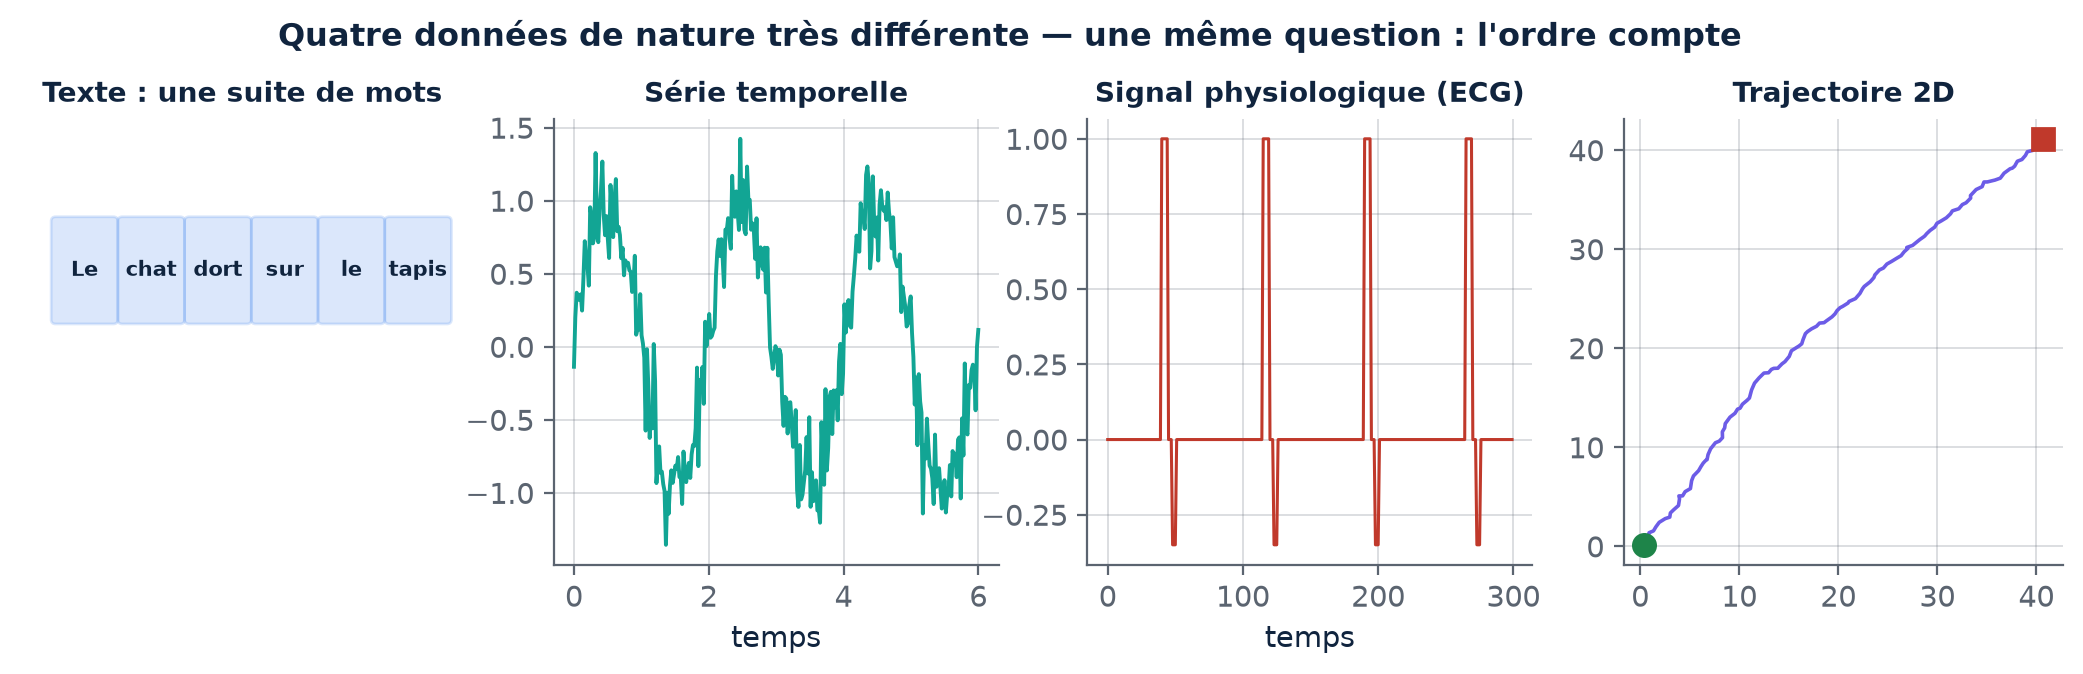
\includegraphics[width=\textwidth]{r01_types_sequences.png}
\end{column}
\begin{column}{0.42\textwidth}
\begin{itemize}
  \item Un texte : une suite de \textbf{mots}.
  \item Une série temporelle : des \textbf{mesures} datées.
  \item Un signal physiologique : un ECG, un capteur.
  \item Une trajectoire : des positions successives.
\end{itemize}
\begin{kbox}[Le dénominateur commun]
Une liste \textbf{ordonnée} d'éléments dont la longueur n'est pas fixée
d'avance.
\end{kbox}
\end{column}
\end{columns}
\end{frame}

\begin{frame}{Même ordre, autre monde}
\begin{columns}[t]
\begin{column}{0.48\textwidth}
\begin{wbox}[Ce que l'on savait faire]
Le CNN prend une image de \textbf{taille fixe} ($28 \times 28$, $32 \times 32$)
et en tire une décision. Les pixels se comptent, la structure est une grille.
\end{wbox}
\begin{wbox}[Ce qui change ici]
\begin{itemize}
  \item La longueur \textbf{varie} d'un exemple à l'autre.
  \item L'ordre porte l'information.
  \item Un mot du début peut gouverner la fin.
\end{itemize}
\end{wbox}
\end{column}
\begin{column}{0.48\textwidth}
\begin{ebox}[Question directe]
Peut-on aplatir une phrase comme on aplatissait une image, et nourrir un MLP ?

\medskip
Non : il faudrait fixer une longueur maximale, et le réseau chercherait des
corrélations entre des positions arbitraires.
\end{ebox}
\end{column}
\end{columns}
\end{frame}

\begin{frame}{Le fil rouge : une trajectoire à prédire}
\begin{columns}[t]
\begin{column}{0.48\textwidth}
\centering
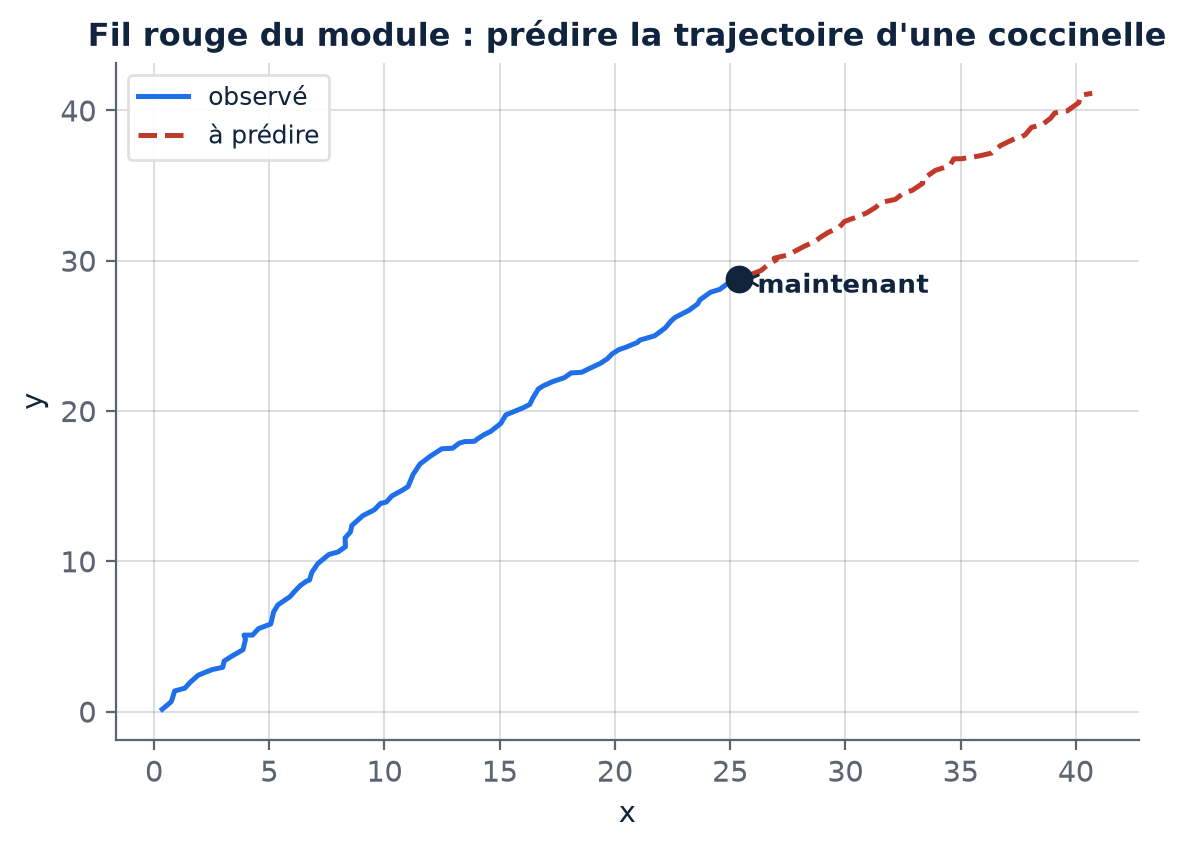
\includegraphics[width=0.46\textwidth]{r08_coccinelle.png}
\end{column}
\begin{column}{0.48\textwidth}
\begin{itemize}
  \item On observe 80 positions de la coccinelle.
  \item On veut prédire les 40 suivantes.
  \item Rien ne fixe la longueur d'avance : la séquence est \textbf{vivante}.
\end{itemize}
\begin{kbox}[Ce qui est demandé]
Utiliser le passé \textbf{comme un tout} --- pas comme une collection de points
indépendants.
\end{kbox}
\end{column}
\end{columns}
\end{frame}

\begin{frame}{Du texte aux nombres : le pipeline}
\begin{center}
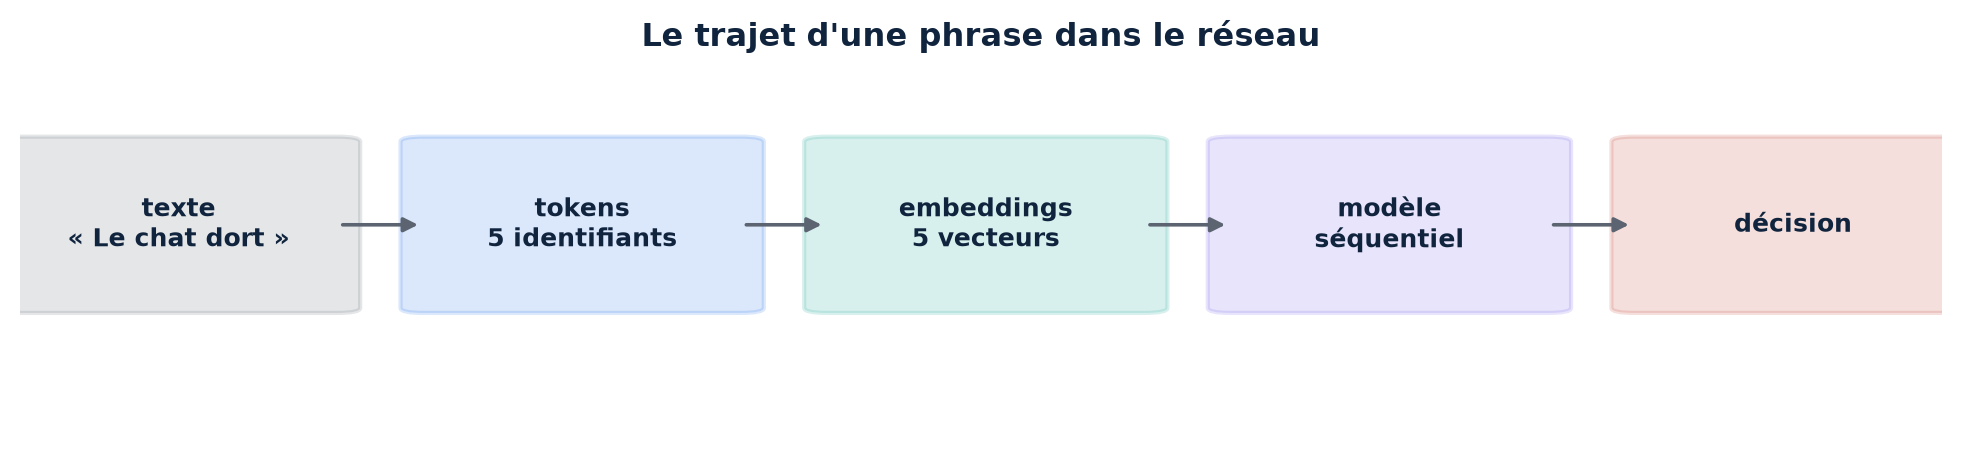
\includegraphics[width=0.94\textwidth]{r07_pipeline_sequence.png}
\end{center}
\vspace{1mm}
\begin{kbox}[Trois étapes obligatoires]
\begin{enumerate}
  \item \textbf{Tokeniser} : découper en unités (mots, sous-mots).
  \item \textbf{Indexer} : chaque unité devient un identifiant entier.
  \item \textbf{Plonger} : chaque identifiant devient un vecteur dense.
\end{enumerate}
\end{kbox}
\end{frame}

\begin{frame}{Quiz d'entrée}
\begin{qbox}[Question 1]
Laquelle de ces données n'est PAS séquentielle au sens de ce module ?
\begin{itemize}
  \item[(a)] une phrase \quad (b) un ECG \quad (c) une photo de chat
\end{itemize}
\end{qbox}
\begin{qbox}[Question 2]
« La souris mange le chat » et « Le chat mange la souris » contiennent les
mêmes mots. Un sac de mots les distingue-t-il ?
\begin{itemize}
  \item[(a)] oui, parfaitement \quad (b) non : l'ordre manque
\end{itemize}
\end{qbox}
\begin{qbox}[Question 3]
Pourquoi le padding est-il nécessaire dans un lot (batch) de séquences ?
\begin{itemize}
  \item[(a)] Pour accélérer \quad (b) Pour donner aux tenseurs une longueur commune
  \quad (c) Pour normaliser
\end{itemize}
\end{qbox}

% [fix] bloc deplace
\end{frame}
\begin{frame}{Quiz d'entrée (suite)}
\begin{solbox}[Réponses]
\textbf{1.} (c) : une image a une taille fixe, pas une suite ordonnée de longueur libre. \quad
\textbf{2.} (b) : le sac de mots détruit l'ordre, donc le sens. \quad
\textbf{3.} (b) : un tenseur doit être rectangulaire ; le masque neutralise le remplissage.
\end{solbox}
\end{frame}

% =====================================================================
%  Chapitre 1 -- Donnees sequentielles
%  Partie b : embeddings, ordre, padding, dependances
% =====================================================================

\begin{frame}{L'embedding : un mot devient un vecteur}
\begin{columns}[t]
\begin{column}{0.50\textwidth}
\centering
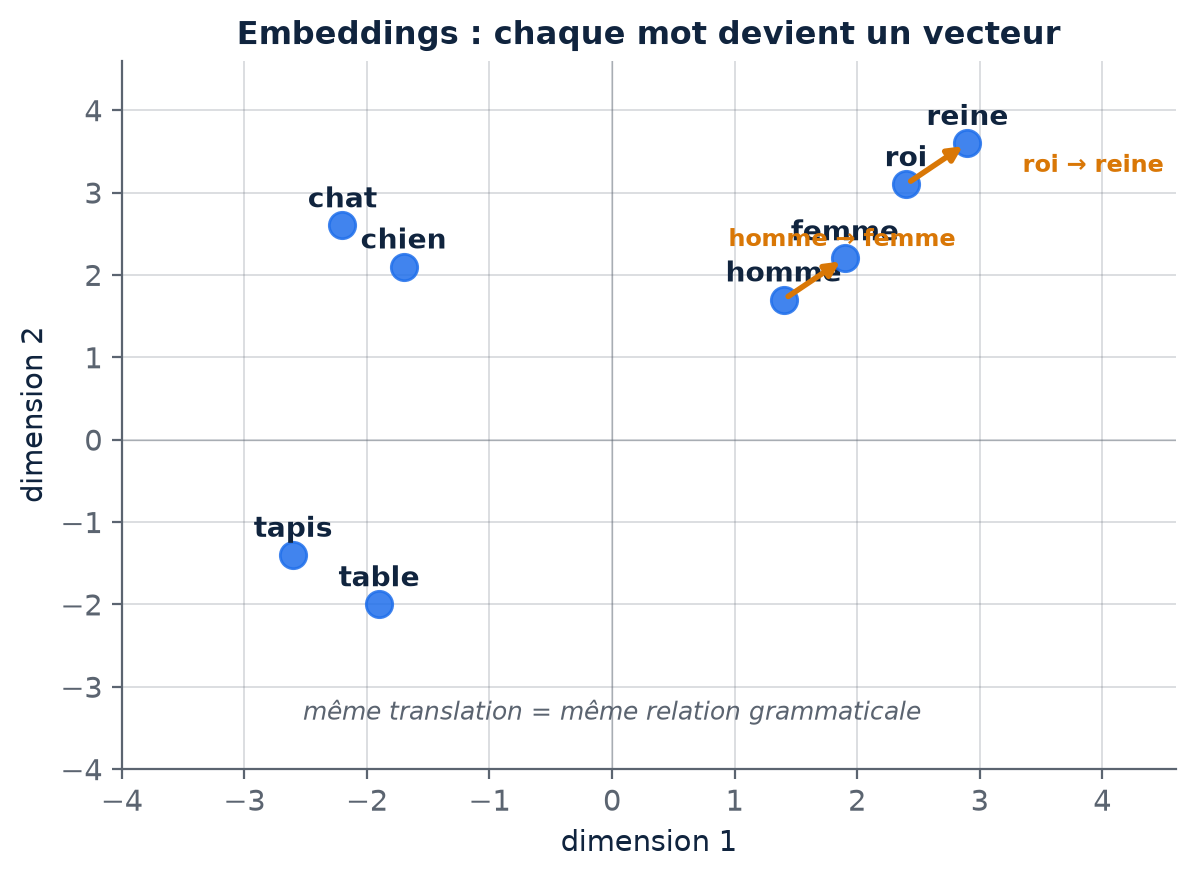
\includegraphics[width=\textwidth]{r02_embeddings.png}
\end{column}
\begin{column}{0.46\textwidth}
\begin{itemize}
  \item Chaque mot du vocabulaire reçoit un vecteur de dimension $d$
  (par exemple $d = 100$).
  \item Ces vecteurs sont \textbf{appris} pendant l'entraînement : les mots qui
  apparaissent dans des contextes voisins finissent voisins.
  \item Une relation grammaticale peut devenir une \textbf{translation} dans
  l'espace.
\end{itemize}
\begin{kbox}[Vocabulaire]
\textbf{Embedding} = table de correspondance
$\text{identifiant} \to \mathbb{R}^{d}$, apprise comme une couche du réseau.
\end{kbox}
\end{column}
\end{columns}
\end{frame}

\begin{frame}[fragile]{En PyTorch : cinq lignes}
\begin{columns}[t]
\begin{column}{0.52\textwidth}
\begin{codebox}[Tokenizer et embedding]
\begin{lstlisting}
import torch, torch.nn as nn

vocab = {"<pad>": 0, "le": 1, "chat": 2,
         "dort": 3, "sur": 4, "tapis": 5}
ids = torch.tensor([vocab[m] for m in
                    "le chat dort".split()])
print(ids)          # tensor([1, 2, 3])

emb = nn.Embedding(6, 4)
print(emb(ids).shape)   # (3, 4)
\end{lstlisting}
\end{codebox}
\end{column}
\begin{column}{0.44\textwidth}
\begin{itemize}
  \item L'identifiant $2$ devient un vecteur de 4 nombres.
  \item Une phrase de 3 mots devient une \textbf{matrice} $3 \times 4$.
  \item Le tenseur d'entrée d'un réseau séquentiel est donc
  $(\text{lot}, \text{longueur}, d)$.
\end{itemize}
\begin{wbox}[Le 0 du padding]
Réserver l'indice 0 pour le padding est une convention : son embedding
sera neutralisé par le masque.
\end{wbox}
\end{column}
\end{columns}
\end{frame}

\begin{frame}{L'ordre porte le sens}
\begin{center}

\includegraphics[width=0.9\textwidth]{r03_ordre_compte.png}
\end{center}
\vspace{1mm}
\begin{solbox}[Conclusion]
Un modèle qui additionne les embeddings des mots (sac de mots) confond ces
deux phrases. \textbf{Le traitement doit être ordonné.}
\end{solbox}
\end{frame}

\begin{frame}{Des longueurs variables dans un même lot}
\begin{center}
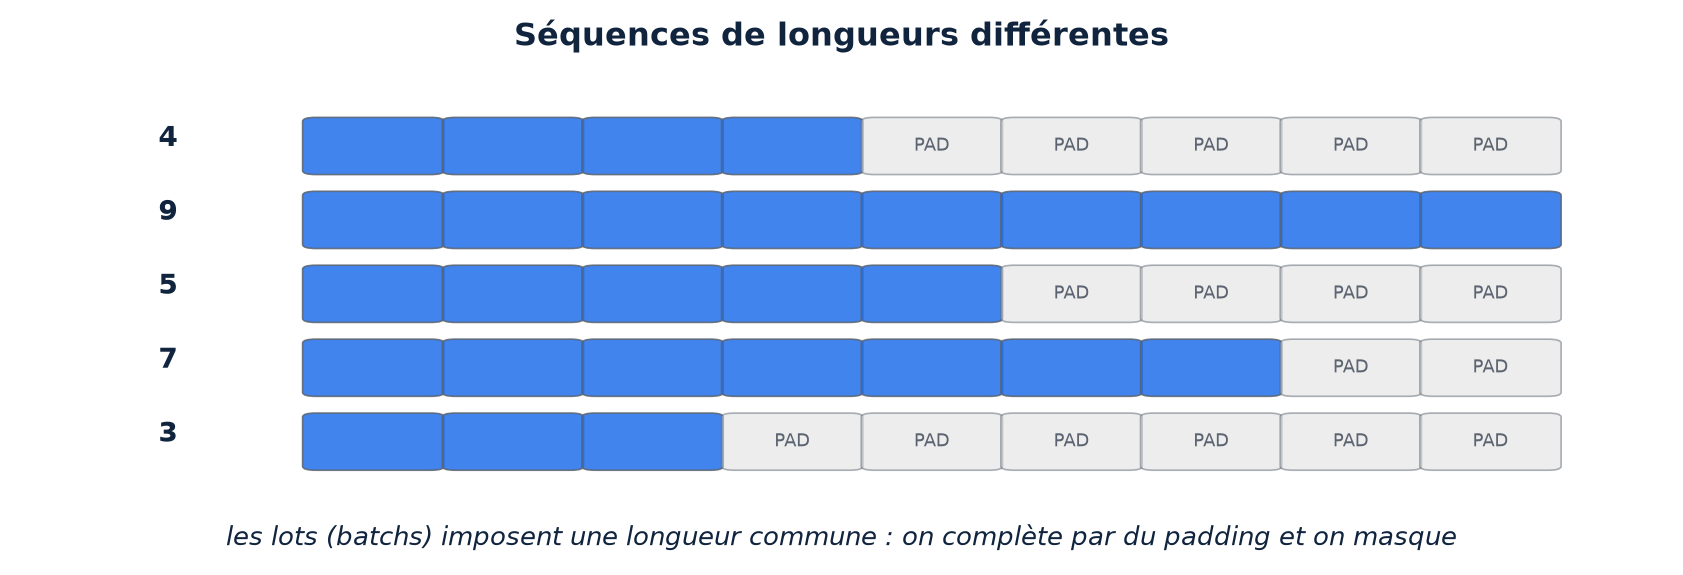
\includegraphics[width=0.9\textwidth]{r04_padding.png}
\end{center}
\vspace{1mm}
\begin{itemize}
  \item On complète avec un \textbf{token de padding} (indice 0).
  \item On fournit au réseau un \textbf{masque} : les positions de padding ne
  contribuent ni à la décision ni à la perte.
\end{itemize}
\begin{wbox}[Le piège classique]
Oublier le masque fausse les moyennes : les phrases courtes pèsent autant
que les longues, et le modèle apprend du bruit.
\end{wbox}
\end{frame}

\begin{frame}{Le vrai obstacle : les dépendances à distance}
\begin{center}
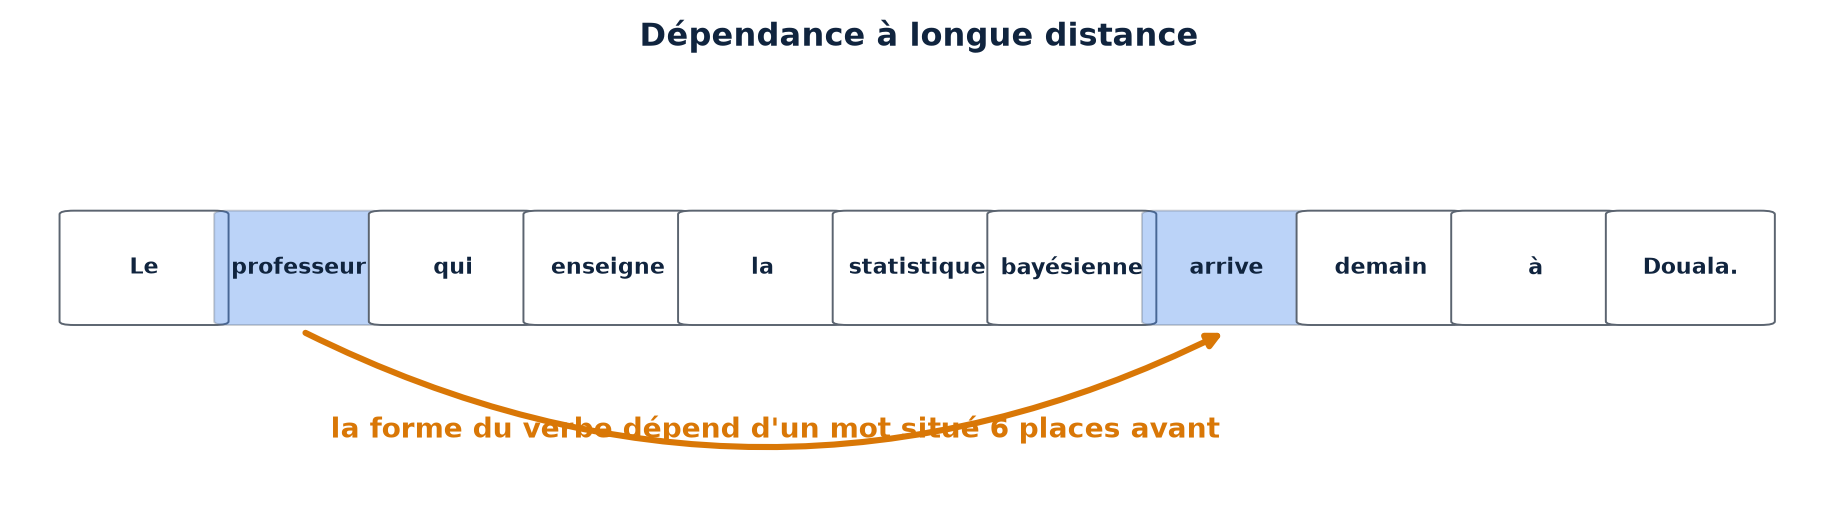
\includegraphics[width=0.94\textwidth]{r05_dependance_distance.png}
\end{center}
\vspace{1mm}
\begin{kbox}[Six places avant]
Ici, « arrive » s'accorde avec « professeur » situé 6 mots avant. Un réseau qui
ne voit qu'une fenêtre courte ne peut pas établir ce lien.
\end{kbox}
\end{frame}

\begin{frame}{Et le CNN, alors ?}
\begin{columns}[t]
\begin{column}{0.52\textwidth}
\centering
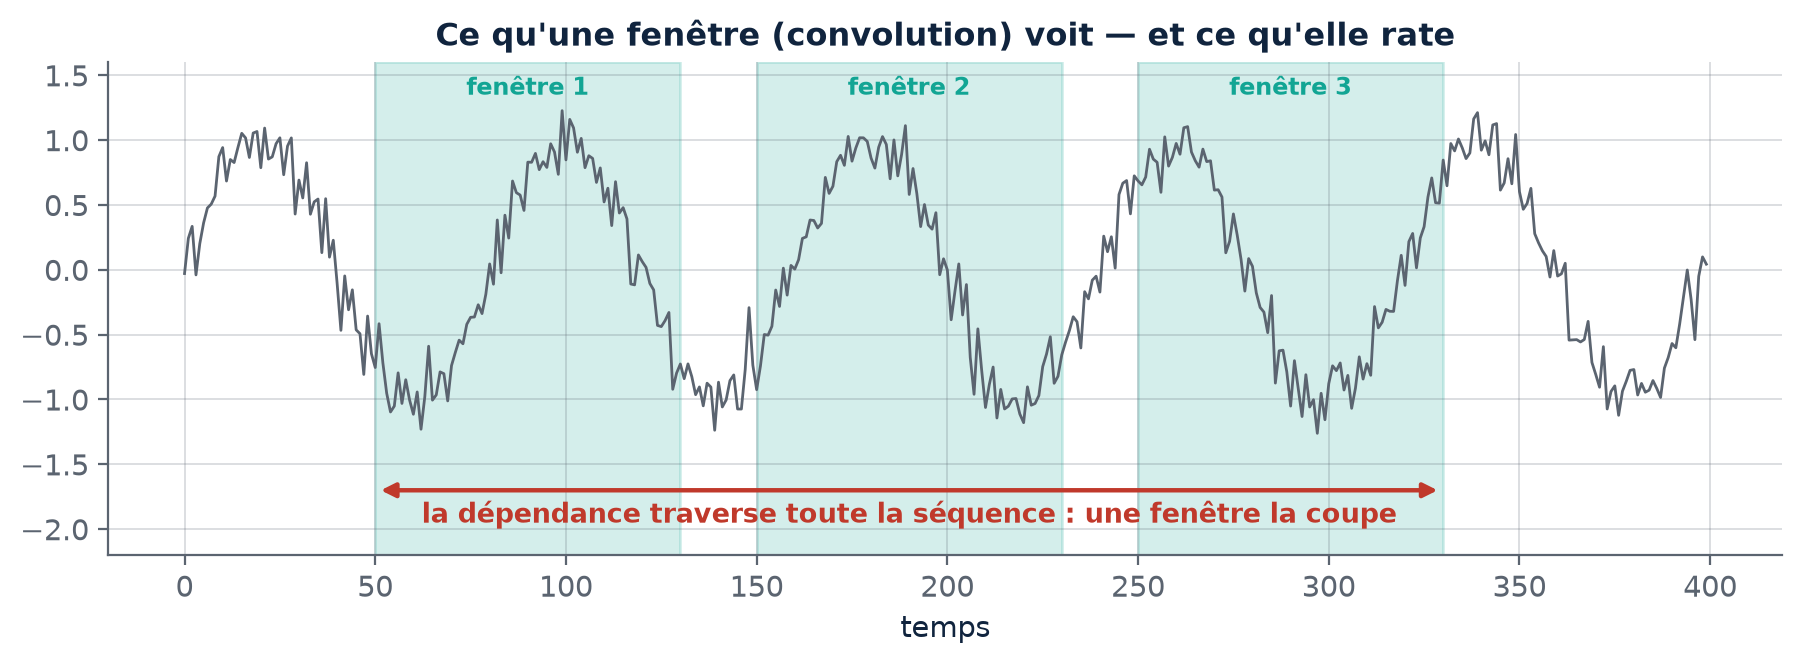
\includegraphics[width=\textwidth]{r06_fenetre_insuffisante.png}
\end{column}
\begin{column}{0.44\textwidth}
\begin{itemize}
  \item Une convolution 1D \textbf{peut} traiter du texte : elle voit des
  n-grammes.
  \item Mais pour relier deux points éloignés, il faut empiler les couches ---
  ou beaucoup de filtres.
  \item Et la longueur variable reste malcommode.
\end{itemize}
\begin{kbox}[Ce qu'il faut]
Un mécanisme qui \textbf{transporte} l'information d'un pas au suivant ---
parce que le réseau \textbf{conserve un état}.
\end{kbox}
\end{column}
\end{columns}
\end{frame}

\begin{frame}{Quiz 1 --- le terrain de jeu}
\begin{qbox}[Question 1]
Un embedding de dimension 100 pour un vocabulaire de 20 000 mots représente :
\begin{itemize}
  \item[(a)] 20 000 paramètres \quad (b) 2 000 000 \quad (c) 100
\end{itemize}
\end{qbox}
\begin{qbox}[Question 2]
Une phrase de 12 mots avec des embeddings de dimension 64 est un tenseur de forme :
\begin{itemize}
  \item[(a)] $(12,)$ \quad (b) $(12, 64)$ \quad (c) $(64, 64)$
\end{itemize}
\end{qbox}
\begin{qbox}[Question 3]
Que fait le masque sur une position de padding ?
\begin{itemize}
  \item[(a)] Il remet le mot à zéro \quad (b) Il retire la position de la décision
  et de la perte \quad (c) Il allonge la séquence
\end{itemize}
\end{qbox}
\begin{solbox}[Réponses]
\textbf{1.} (b) : $20\,000 \times 100$ poids, plus rien d'autre. \quad
\textbf{2.} (b) : longueur × dimension. \quad
\textbf{3.} (b) : c'est le masque, pas la mise à zéro seule, qui compte.
\end{solbox}
\end{frame}

\begin{frame}{À retenir et TP}
\begin{kbox}[Les trois idées du chapitre 1]
\begin{enumerate}
  \item Une donnée séquentielle est une liste \textbf{ordonnée} de longueur libre.
  \item Le texte devient un tenseur : tokens $\to$ identifiants $\to$ embeddings.
  \item Ordre et dépendances à distance exigent un mécanisme \textbf{récurrent} :
  un état qui se transporte.
\end{enumerate}
\end{kbox}
\vspace{1.5mm}
\begin{abox}[TP1 : \file{notebooks/TP1_embeddings_sequences.ipynb}]
Construire le vocabulaire, indexer, plonger, padder et masquer --- sur un petit corpus
de critiques. Durée conseillée : \textbf{1 h 30} · barème : \textbf{10 points}.
\end{abox}
\end{frame}

% =====================================================================
%  Chapitre 2 -- Le RNN : architecture et propagation
%  Partie a : deroulement, cellule, etat cache, BPTT
% =====================================================================
\section{Chapitre 2 --- Architecture RNN}

\chapterslide{Chapitre 2}{Le RNN : architecture et propagation}%
{6 h --- déroulement temporel, cellule, BPTT, gradients}%
{\textbf{Objectifs.} Écrire les équations d'une cellule récurrente ; comprendre le
déroulement temporel et la réutilisation des poids ; dérouler la rétropropagation
à travers le temps ; expliquer le gradient qui s'évanouit par le calcul.}

\begin{frame}{L'idée en une phrase}
\begin{kbox}[Une cellule, un état, beaucoup de pas]
Le réseau ne change pas d'un pas de temps à l'autre : c'est la \textbf{même
cellule}, avec les \textbf{mêmes poids}, appliquée successivement à chaque
élément de la séquence.

\medskip
Entre deux pas, elle transmet un \textbf{état caché} $h_t$ --- sa mémoire de
ce qu'elle a déjà lu.
\end{kbox}
\vspace{2mm}
\begin{wbox}[Ce que cela implique]
Le nombre de paramètres ne dépend pas de la longueur de la séquence :
une phrase de 5 mots et une de 500 passent par le même réseau.
\end{wbox}
\end{frame}

\begin{frame}{Le déroulement temporel (unrolling)}
\begin{center}
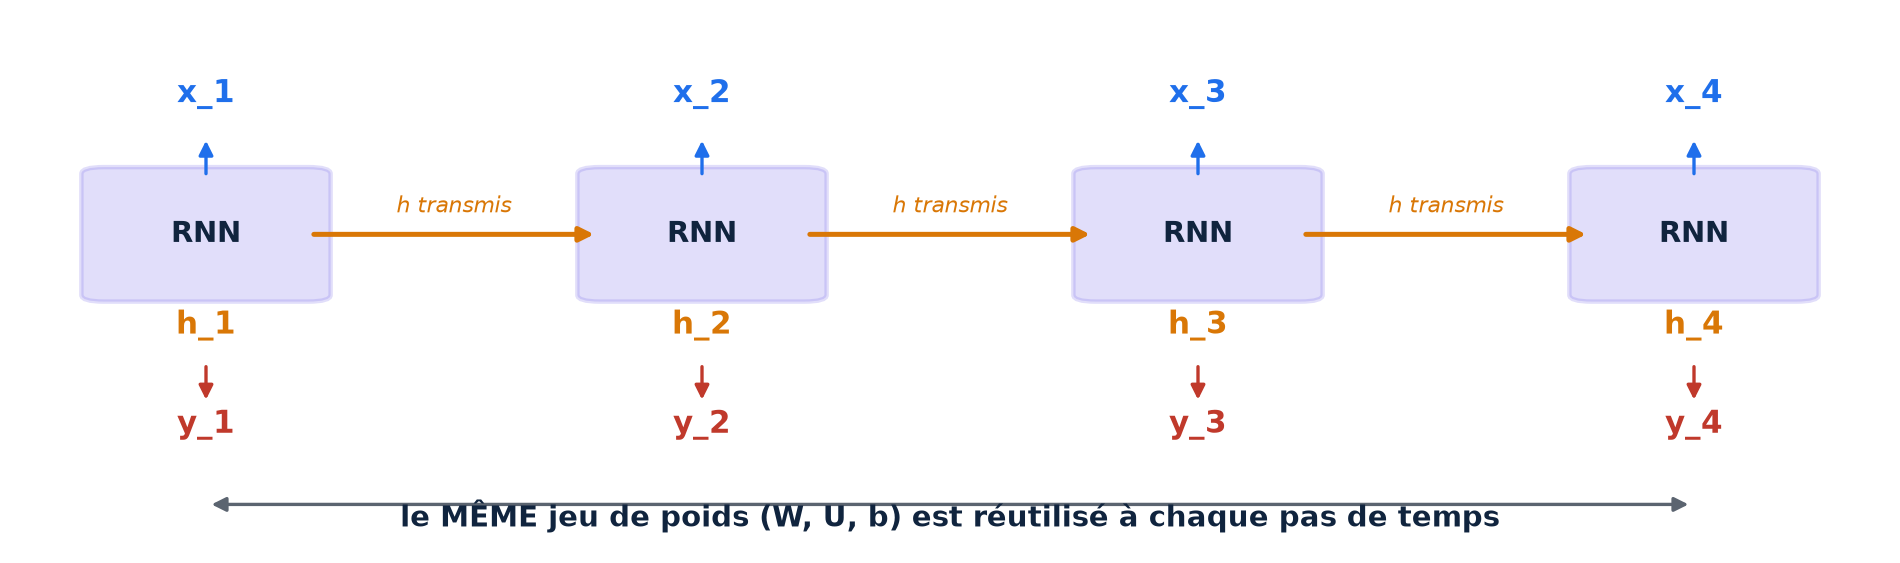
\includegraphics[width=0.95\textwidth]{s01_deroulement.png}
\end{center}
\vspace{1mm}
\begin{itemize}
  \item À gauche : une boucle. À droite : la même chose, déroulée dans le temps.
  \item Les boîtes sont \textbf{la même} cellule : mêmes poids, même biais.
  \item Le trait orange est l'état caché transmis.
\end{itemize}
\end{frame}

\begin{frame}[fragile]{La cellule, en une équation et cinq lignes}
\begin{columns}[t]
\begin{column}{0.48\textwidth}
\begin{codebox}[PyTorch, à la main]
\begin{lstlisting}
def cellule(x_t, h_pre):
    return torch.tanh(
        Wx @ x_t + Wh @ h_pre + b)

h = torch.zeros(H)
for x_t in sequence:
    h = cellule(x_t, h)
\end{lstlisting}
\end{codebox}
\end{column}
\begin{column}{0.48\textwidth}
\begin{center}
$h_t = \tanh(W_x\, x_t + W_h\, h_{t-1} + b)$
\end{center}
\vspace{1mm}
\begin{itemize}
  \item $W_x$ : comment l'entrée du pas pénètre.
  \item $W_h$ : comment la mémoire se maintient.
  \item $\tanh$ : garde $h_t$ dans $[-1, 1]$.
\end{itemize}
\end{column}
\end{columns}
\end{frame}

\begin{frame}{L'état caché en action}
\begin{center}
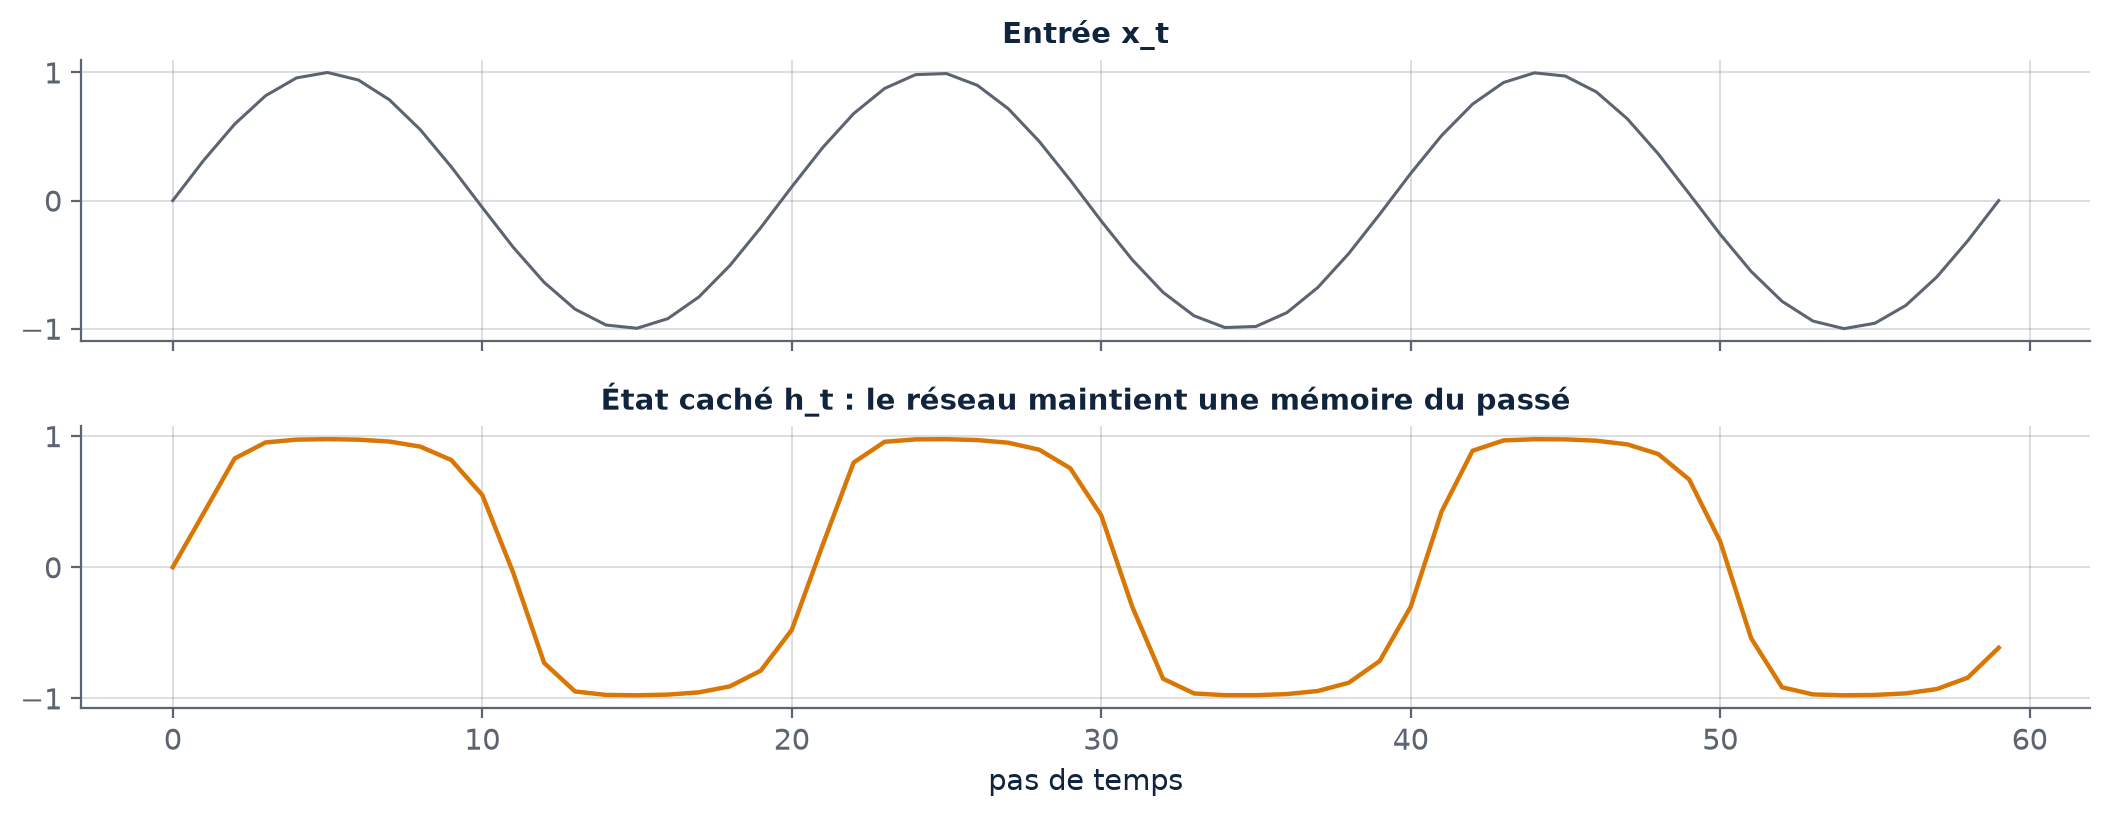
\includegraphics[width=0.88\textwidth]{s03_etat_cache.png}
\end{center}
\vspace{1mm}
\begin{kbox}[Une mémoire vivante]
L'état $h_t$ suit l'entrée, la lisse, la retarde : il encode un \textbf{résumé
mobile} de tout ce qui a été vu jusqu'ici.
\end{kbox}
\end{frame}

\begin{frame}{Combien de paramètres ?}
\begin{columns}[t]
\begin{column}{0.96\textwidth}
\begin{itemize}
  \item Une couche RNN : $E \times H + H \times H + H$ paramètres
  (entrée, récurrence, biais).
  \item \textbf{Aucun} terme ne dépend de la longueur $T$.
  \item La même matrice $W_h$ s'applique $T$ fois : c'est le partage de poids
  du CNN, version temporelle.
\end{itemize}
\begin{solbox}[Repère du cours]
$E = 300$, $H = 128$ : $300 \times 128 + 128 \times 128 + 128
= 54\,784$ paramètres.
\end{solbox}
\end{column}
\end{columns}
% [fix] figure sortie
\end{frame}

\begin{frame}{Combien de paramètres ? --- la figure}\begin{center}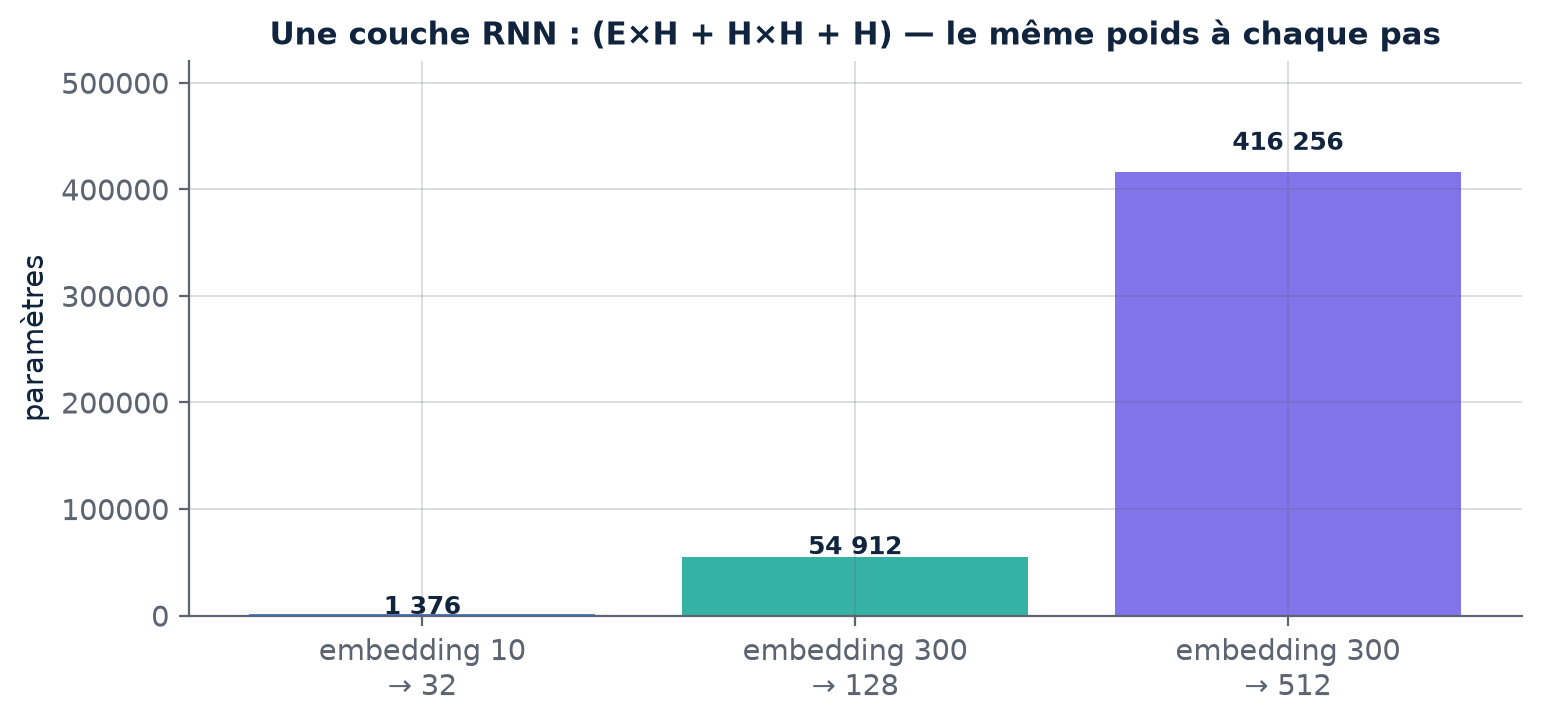
\includegraphics[width=.92\textwidth]{s09_parametres.png}\end{center}\end{frame}

\begin{frame}{Entraîner : la rétropropagation à travers le temps}
\begin{center}
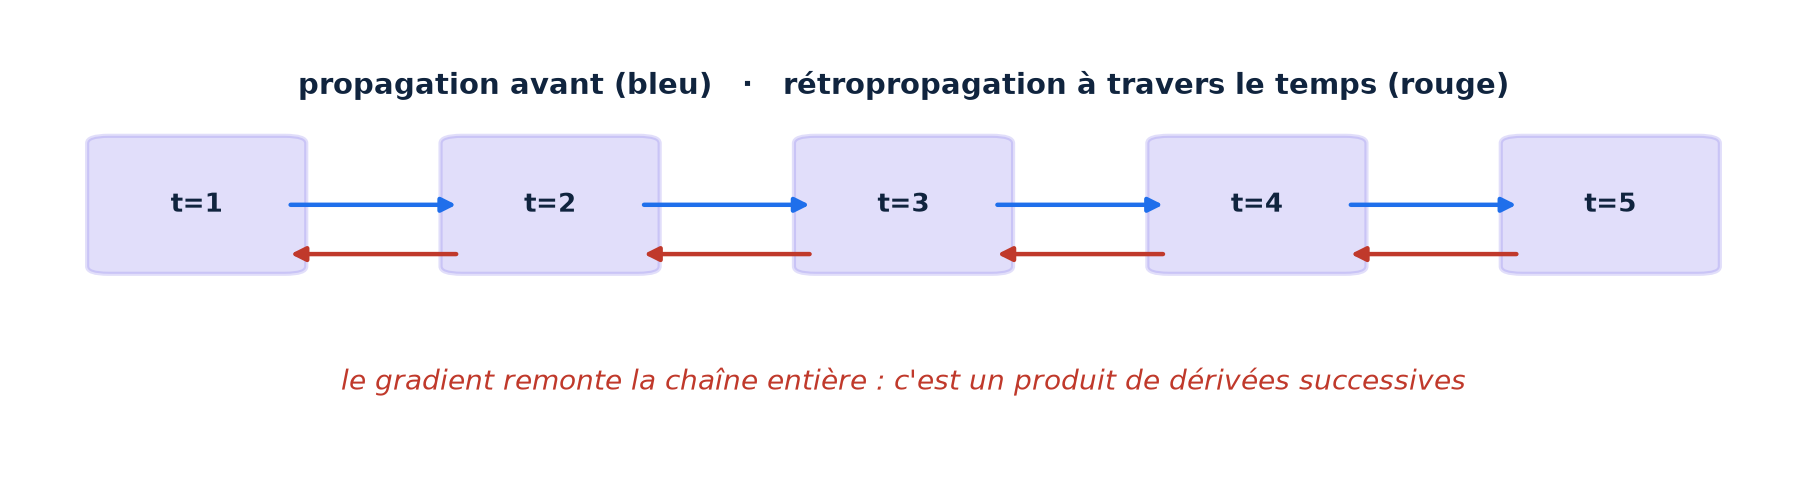
\includegraphics[width=0.94\textwidth]{s04_bptt.png}
\end{center}
\vspace{1mm}
\begin{itemize}
  \item On déroule, on calcule la perte, puis le gradient \textbf{remonte}
  la chaîne dans le sens inverse du temps.
  \item Le gradient qui atteint le pas 1 a traversé \textbf{tous} les pas
  intermédiaires.
\end{itemize}
\end{frame}

\begin{frame}{Le problème, formulé proprement}
\begin{columns}[t]
\begin{column}{0.52\textwidth}
\begin{kbox}[Le gradient le long du temps]
Pour remonter $T$ pas, le gradient contient un produit :
\[
\frac{\partial h_t}{\partial h_0}
\approx \prod_{k=1}^{t} W_h^{\,\top} \operatorname{diag}(\tanh')
\]
\end{kbox}
\begin{itemize}
  \item Si la norme de chaque facteur vaut $< 1$ : le produit tend vers 0
  --- gradient \textbf{évanouissant}.
  \item Si elle vaut $> 1$ : le produit explose.
\end{itemize}
\end{column}
\begin{column}{0.44\textwidth}
\begin{wbox}[Ni l'un ni l'autre n'est bon]
\begin{itemize}
  \item Évanouissant : le réseau \textbf{oublie} le début de la séquence.
  \item Explosant : les mises à jour détruisent les poids.
\end{itemize}
Le chapitre 3 règle le premier cas ; le clipping règle le second.
\end{wbox}
\end{column}
\end{columns}
\end{frame}

\begin{frame}{La preuve par le calcul}
\begin{columns}[t]
\begin{column}{0.96\textwidth}
\begin{itemize}
  \item Chaque courbe est un \textbf{calcul exact} : $r^{t}$ pour un rayon
  spectral $r$ de la matrice de récurrence.
  \item $r = 0{,}55$ : après 20 pas, il reste $0{,}55^{20} \approx 6 \times
  10^{-6}$ du gradient.
  \item $r = 1{,}35$ : après 20 pas, $\approx 406$ — et cela continue.
\end{itemize}
\begin{solbox}[Repères du cours]
$r = 0{,}55$ : $r^{20} = 6{,}4 \cdot 10^{-6}$ ;\quad
$r = 1{,}35$ : $r^{20} = 405{,}9$.
\end{solbox}
\end{column}
\end{columns}
% [fix] figure sortie
\end{frame}

\begin{frame}{La preuve par le calcul --- la figure}\begin{center}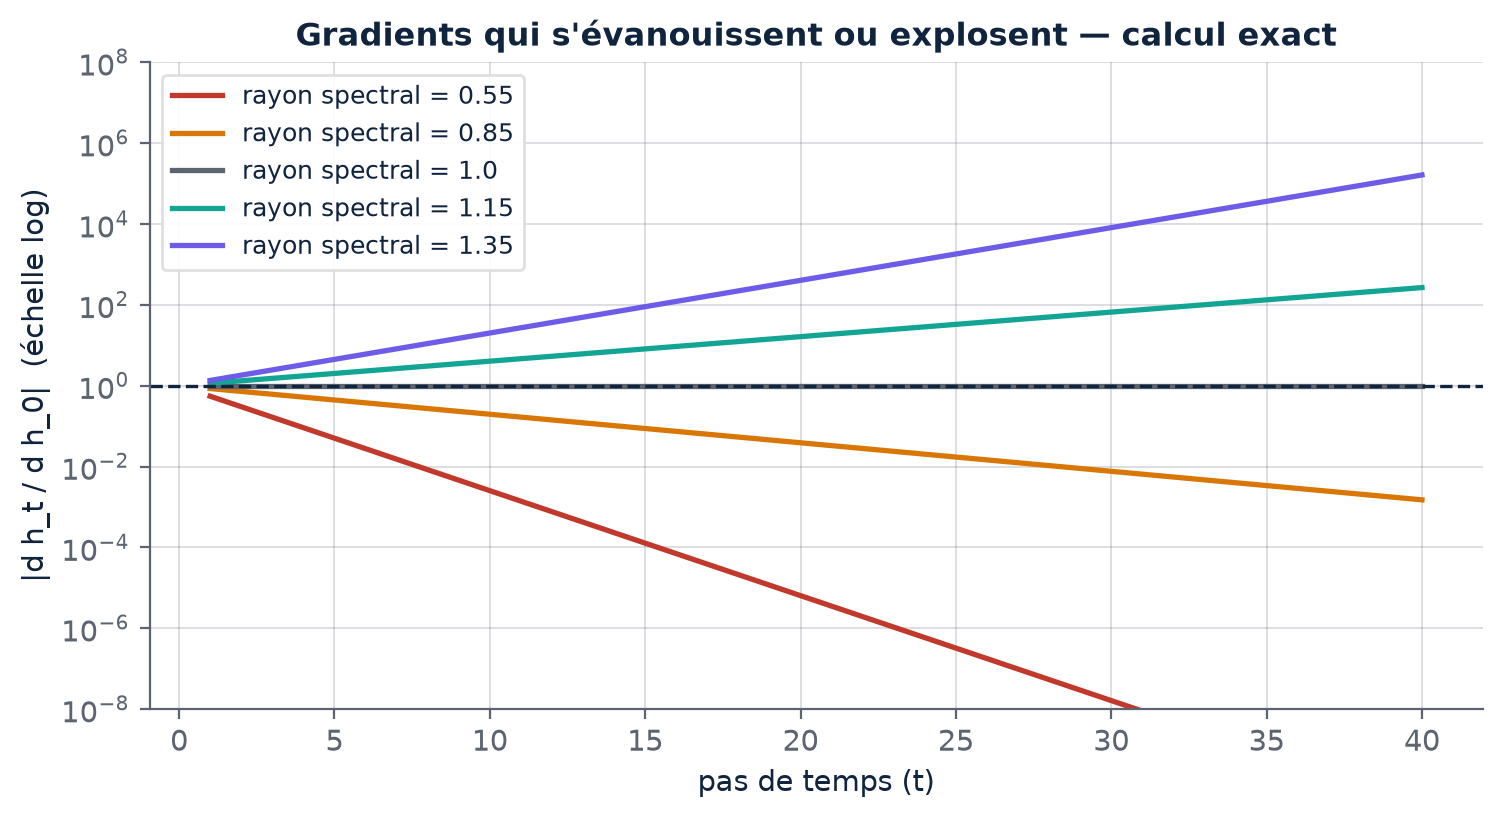
\includegraphics[width=.92\textwidth]{s05_gradients.png}\end{center}\end{frame}

\begin{frame}{Le clipping : traiter l'explosion}
\begin{center}
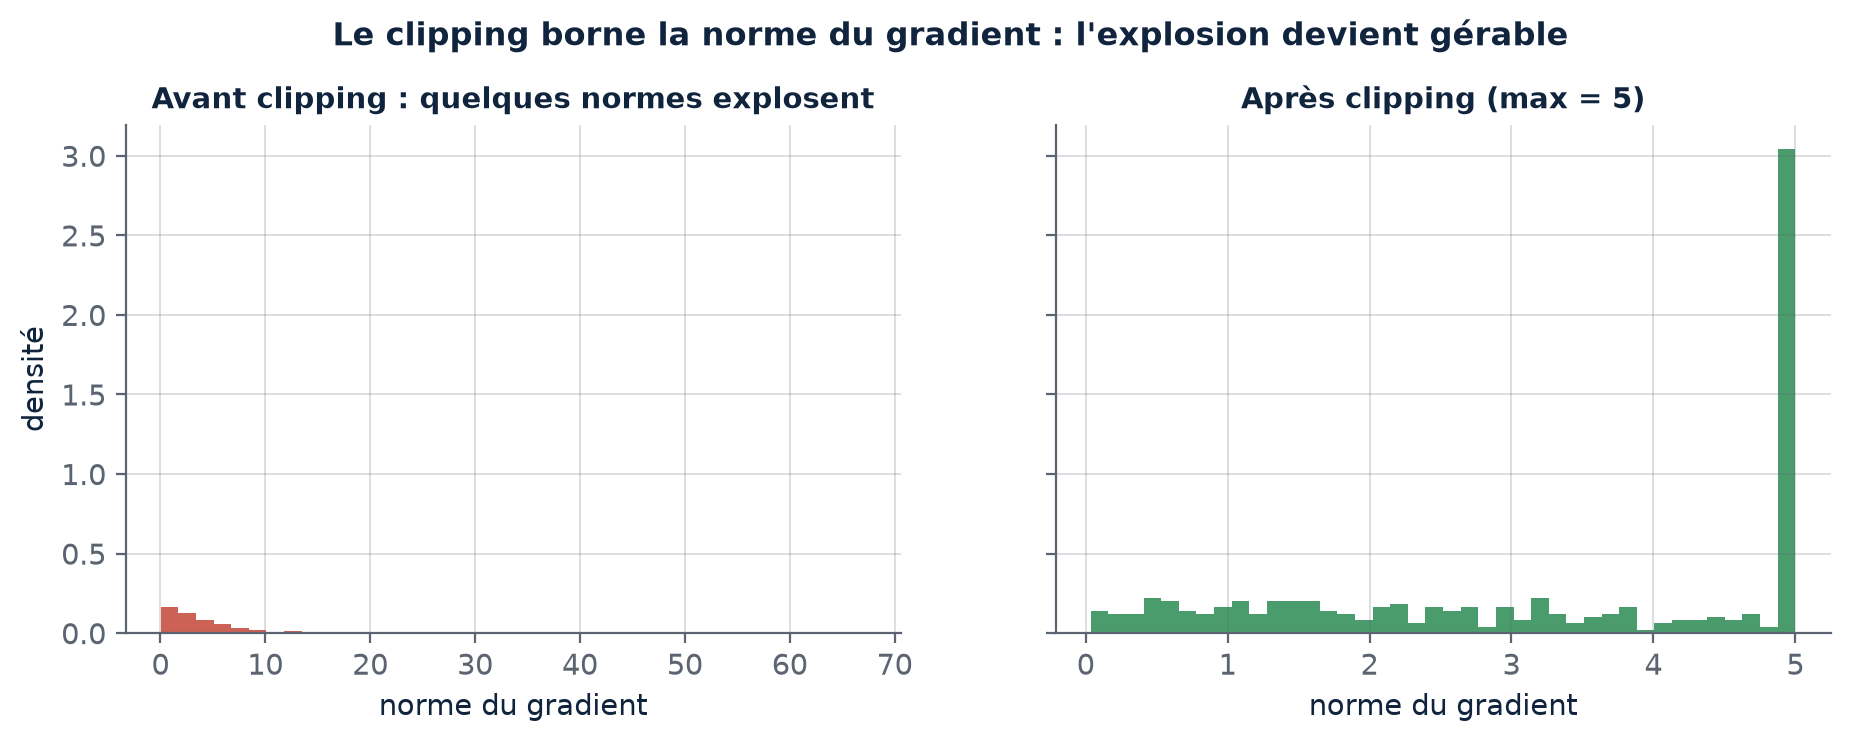
\includegraphics[width=0.86\textwidth]{s06_clipping.png}
\end{center}
\vspace{1mm}
\begin{itemize}
  \item On mesure la \textbf{norme} du gradient ; si elle dépasse un seuil
  (typiquement 5), on la ramène à ce seuil.
  \item Une ligne de code, un geste réflexe : \py{torch.nn.utils.clip_grad_norm_}.
\end{itemize}
\end{frame}

% =====================================================================
%  Chapitre 2 -- Le RNN
%  Partie b : formes d'entree/sortie, seq2seq, quiz, TP2
% =====================================================================

\begin{frame}{Une même cellule, plusieurs usages}
\begin{center}
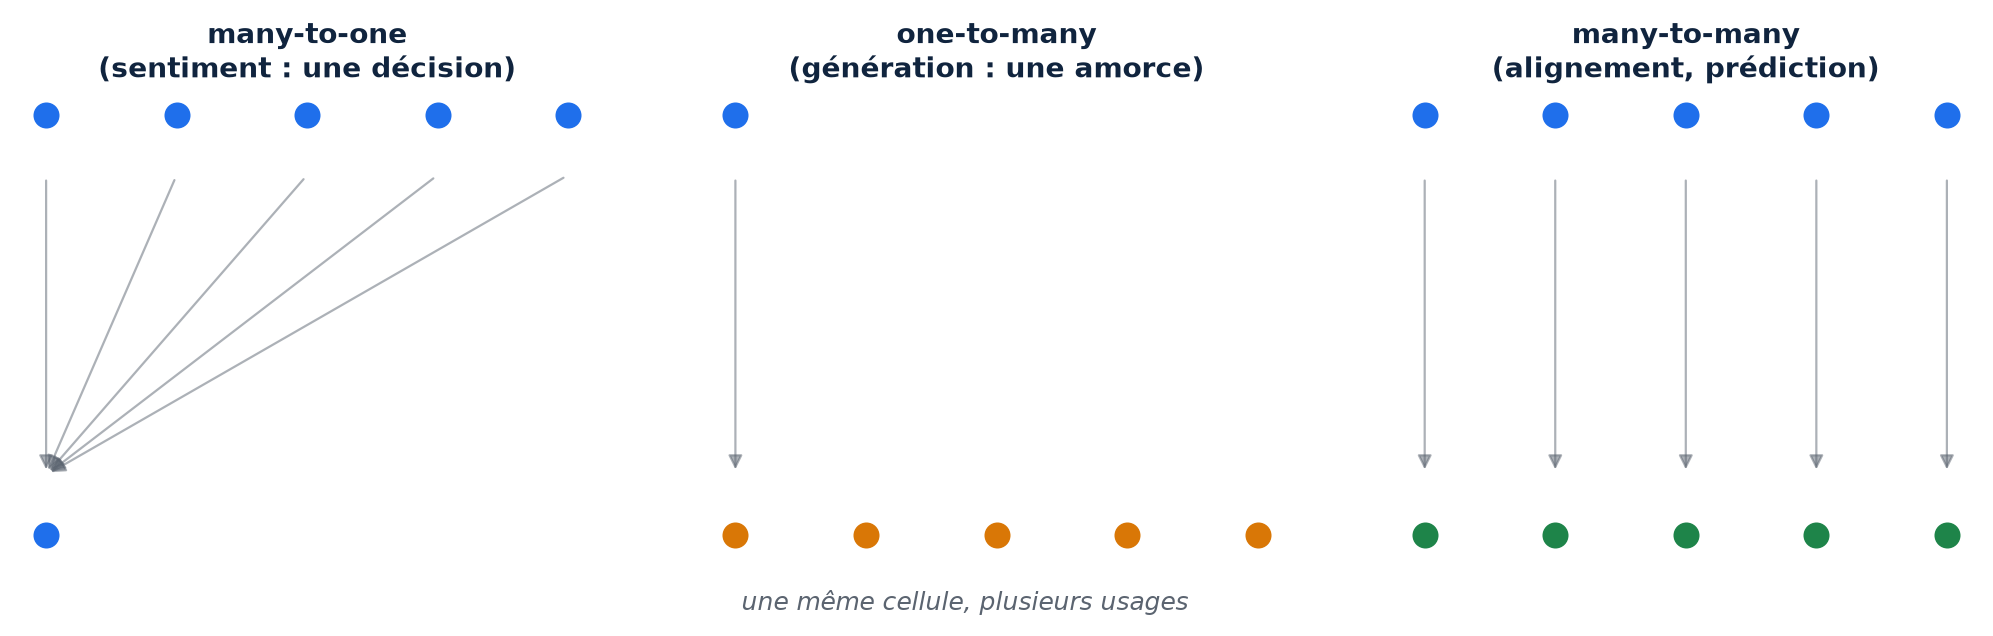
\includegraphics[width=0.95\textwidth]{s07_formes_es.png}
\end{center}
\vspace{1mm}
\begin{columns}[t]
\begin{column}{0.32\textwidth}
\begin{ebox}[many-to-one]
Lire toute une critique, décider une fois : \textbf{sentiment}.
\end{ebox}
\end{column}
\begin{column}{0.32\textwidth}
\begin{ebox}[one-to-many]
Une amorce, puis générer une suite : \textbf{texte}.
\end{ebox}
\end{column}
\begin{column}{0.32\textwidth}
\begin{ebox}[many-to-many]
Un pas, une sortie : \textbf{étiquetage}, prédiction pas à pas.
\end{ebox}
\end{column}
\end{columns}
\end{frame}

\begin{frame}{Seq2seq : traduire, résumer, transcrire}
\begin{center}
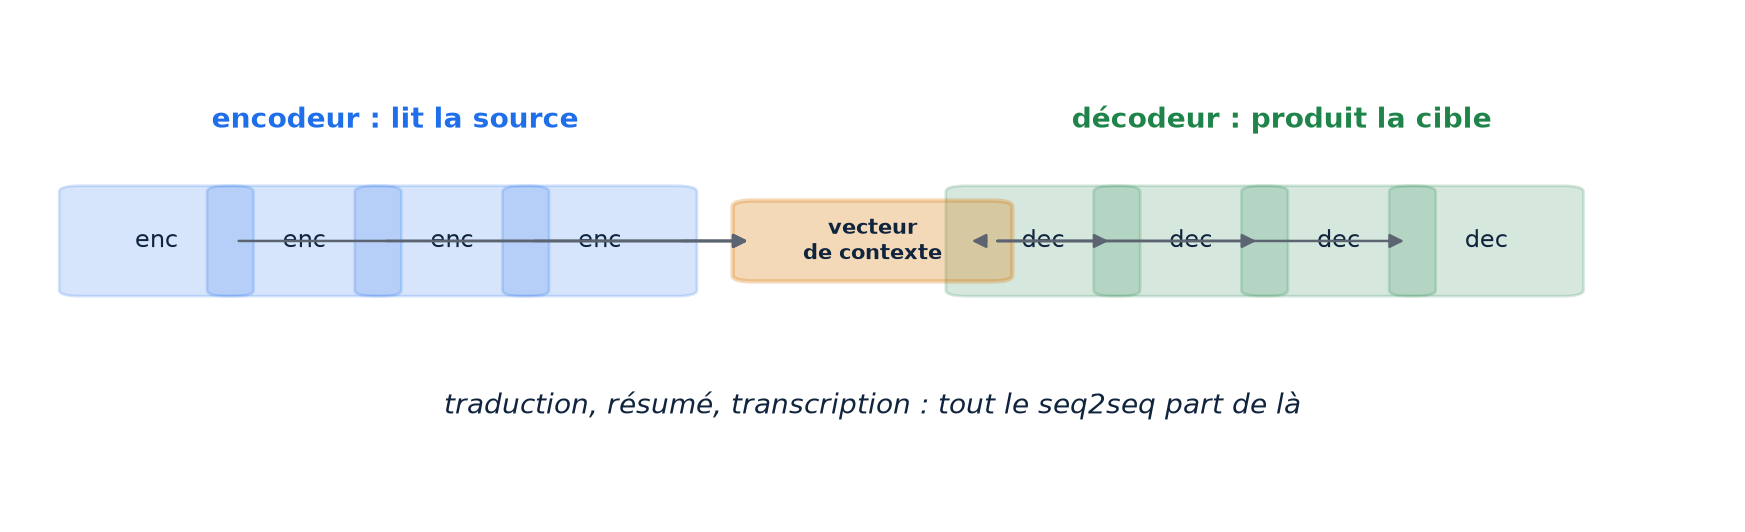
\includegraphics[width=0.9\textwidth]{s08_seq2seq.png}
\end{center}
\vspace{1mm}
\begin{itemize}
  \item L'\textbf{encodeur} lit la source et condense tout dans un vecteur
  de contexte.
  \item Le \textbf{décodeur} produit la cible à partir de ce vecteur.
\end{itemize}
\begin{wbox}[Le goulot d'étranglement]
Tout le contenu de la source passe par un vecteur unique : pour les longues
séquences, c'est insuffisant --- d'où l'attention (chapitre 3).
\end{wbox}
\end{frame}

\begin{frame}[fragile]{Seq2seq en pratique : le décodeur génère mot à mot}
\begin{columns}[t]
\begin{column}{0.52\textwidth}
\begin{itemize}
  \item À chaque pas, le décodeur produit une \textbf{distribution}
  sur le vocabulaire (softmax).
  \item On choisit le mot le plus probable --- ou l'on échantillonne
  (chapitre 4).
  \item Ce mot devient l'entrée du pas suivant.
\end{itemize}
\end{column}
\begin{column}{0.44\textwidth}
\begin{codebox}[Boucle de génération]
\begin{lstlisting}
h = contexte
mot = "<debut>"
while mot != "<fin>":
    logits = decodeur(mot, h)
    mot = vocab[int(logits.argmax())]
    sortie.append(mot)
\end{lstlisting}
\end{codebox}
\end{column}
\end{columns}
\end{frame}

\begin{frame}{Quiz 2 --- le RNN}
\begin{qbox}[Question 1]
Le nombre de paramètres d'une couche RNN dépend-il de la longueur $T$ des séquences ?
\begin{itemize}
  \item[(a)] oui, linéairement \quad (b) non, jamais \quad (c) oui, en $T^2$
\end{itemize}
\end{qbox}
\begin{qbox}[Question 2]
Avec un rayon spectral $r = 0{,}55$, combien reste-t-il du gradient après 20 pas ?
\begin{itemize}
  \item[(a)] $\approx 0{,}55$ \quad (b) $\approx 6 \times 10^{-6}$
  \quad (c) $\approx 406$
\end{itemize}
\end{qbox}
\begin{qbox}[Question 3]
Le clipping de gradient traite…
\begin{itemize}
  \item[(a)] l'évanouissement \quad (b) l'explosion \quad (c) les deux
\end{itemize}
\end{qbox}
\begin{qbox}[Question 4]
Classer une critique en positive/négative est une tâche…
\begin{itemize}
  \item[(a)] one-to-many \quad (b) many-to-one \quad (c) many-to-many
\end{itemize}
\end{qbox}

% [fix] bloc deplace
\end{frame}
\begin{frame}{Quiz 2 --- le RNN (suite)}
\begin{solbox}[Réponses]
\textbf{1.} (b) : le partage de poids est total. \quad
\textbf{2.} (b) : $0{,}55^{20} = 6{,}4 \cdot 10^{-6}$. \quad
\textbf{3.} (b) : on borne la norme. \quad
\textbf{4.} (b) : toute la séquence, une seule décision.
\end{solbox}
\end{frame}

\begin{frame}{À retenir et TP}
\begin{kbox}[Les trois idées du chapitre 2]
\begin{enumerate}
  \item Une \textbf{cellule unique} déroulée dans le temps : mêmes poids
  à chaque pas, état caché transmis.
  \item $h_t = \tanh(W_x x_t + W_h h_{t-1} + b)$ --- tout est là.
  \item Le gradient le long du temps est un \textbf{produit} : évanescence
  ou explosion, selon le rayon spectral.
\end{enumerate}
\end{kbox}
\vspace{1.5mm}
\begin{abox}[TP2 : \file{notebooks/TP2_RNN_serie_temporelle.ipynb}]
Coder la cellule à la main, vérifier l'évanouissement du gradient, puis entraîner
un RNN à prédire la suite d'une série. Durée : \textbf{2 h} · barème : \textbf{10 points}.
\end{abox}
\end{frame}

% =====================================================================
%  Chapitre 3 -- LSTM et GRU : dompter la memoire
%  Partie a : la cellule LSTM, ses portes, le convoyeur
% =====================================================================
\section{Chapitre 3 --- LSTM et GRU}

\chapterslide{Chapitre 3}{LSTM et GRU : dompter la mémoire}%
{5 h --- portes, état de cellule, survie du gradient, variantes}%
{\textbf{Objectifs.} Nommer et expliquer les trois portes du LSTM ; comprendre
pourquoi l'état de cellule laisse passer le gradient ; comparer LSTM et GRU ;
situer le bidirectionnel et l'empilement.}

\begin{frame}{Le diagnostic du chapitre 2}
\begin{columns}[t]
\begin{column}{0.48\textwidth}
\begin{wbox}[Le RNN simple oublie]
Sa mémoire est réécrite à \textbf{chaque pas} : $h_t = \tanh(\ldots)$ écrase
$h_{t-1}$ entièrement. Après quelques dizaines de pas, le début de la séquence
a disparu.
\end{wbox}
\begin{wbox}[Et le gradient avec]
Le produit des dérivées s'effondre : le réseau ne peut pas apprendre une
dépendance à 30 pas de distance.
\end{wbox}
\end{column}
\begin{column}{0.48\textwidth}
\begin{kbox}[L'intuition de la solution]
Et si, au lieu de tout réécrire, on ajoutait un \textbf{chemin protégé} qui
transporte l'information, avec des \textbf{portes} qui décident quoi garder,
quoi écrire, quoi dévoiler ?
\end{kbox}
\begin{solbox}[C'est exactement le LSTM (1997)]
Hochreiter et Schmidhuber : \textbf{Long Short-Term Memory}. La idée tient en
un mot : un \emph{convoyeur}.
\end{solbox}
\end{column}
\end{columns}
\end{frame}

\begin{frame}{La cellule LSTM, en un coup d'œil}
\begin{center}
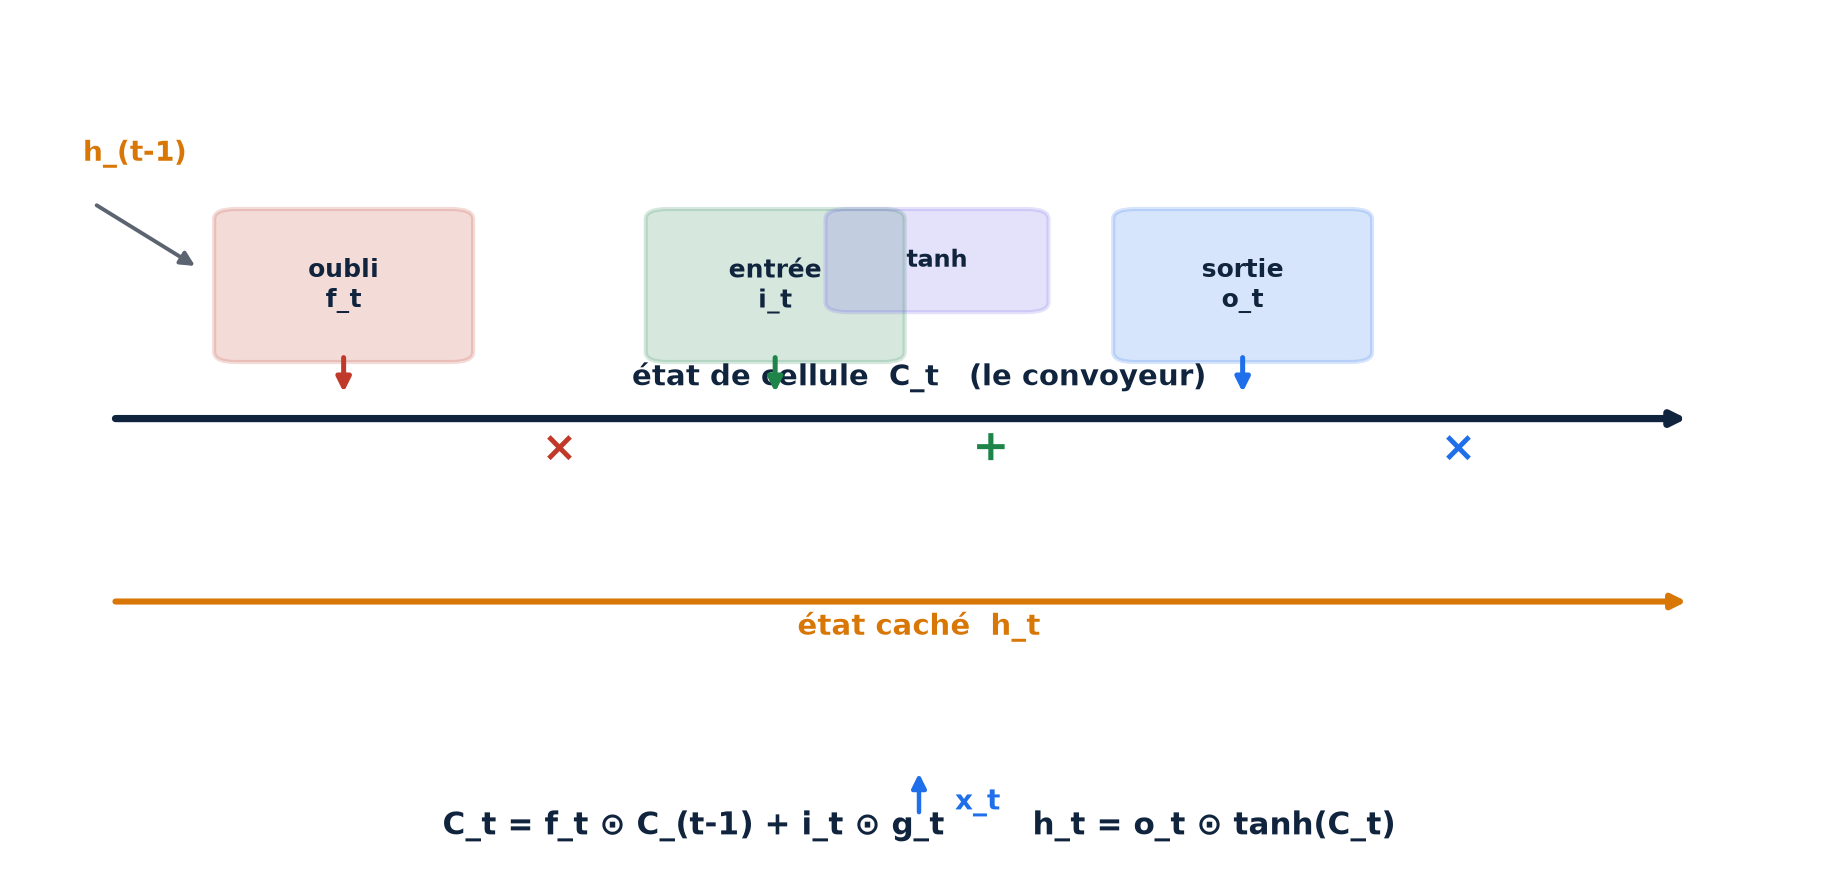
\includegraphics[width=0.95\textwidth]{t01_lstm_cellule.png}
\end{center}
\end{frame}

\begin{frame}{Les trois portes, une par une}
\begin{columns}[t]
\begin{column}{0.32\textwidth}
\begin{wbox}[Porte d'oubli $f_t$]
Vaut entre 0 et 1 à chaque pas : 0 = jeter, 1 = garder.

« Quand un nouveau sujet commence, oublie l'ancien. »
\end{wbox}
\end{column}
\begin{column}{0.32\textwidth}
\begin{wbox}[Porte d'entrée $i_t$]
Combien de la \textbf{nouvelle} information écrire dans l'état.

« Ce mot compte : range-le. »
\end{wbox}
\end{column}
\begin{column}{0.32\textwidth}
\begin{wbox}[Porte de sortie $o_t$]
Combien de l'état \textbf{révéler} à la sortie.

« Garde-le en mémoire, mais ne le montre pas encore. »
\end{wbox}
\end{column}
\end{columns}
\vspace{2mm}
\begin{kbox}[Toutes les portes sont apprises]
Chaque porte est une couche sigmoïde sur $[x_t, h_{t-1}]$ : le réseau apprend
\emph{quand} ouvrir et fermer. Ce n'est pas de la logique codée à la main.
\end{kbox}
\end{frame}

\begin{frame}{Les équations, commentées}
\begin{center}
\small
\begin{tabular}{@{}lll@{}}
\toprule
\textbf{Porte / état} & \textbf{Formule} & \textbf{Rôle} \\
\midrule
oubli & $f_t = \sigma(W_f[x_t, h_{t-1}] + b_f)$ & garder l'ancien \\
entrée & $i_t = \sigma(W_i[x_t, h_{t-1}] + b_i)$ & accepter le nouveau \\
candidat & $\tilde{C}_t = \tanh(W_C[x_t, h_{t-1}] + b_C)$ & ce qu'on proposerait \\
\textbf{état} & $C_t = f_t \odot C_{t-1} + i_t \odot \tilde{C}_t$ & \textbf{mise à jour} \\
sortie & $o_t = \sigma(W_o[x_t, h_{t-1}] + b_o)$ & combien montrer \\
sortie cachée & $h_t = o_t \odot \tanh(C_t)$ & ce que le réseau publie \\
\bottomrule
\end{tabular}
\end{center}
\vspace{1mm}
\begin{kbox}[La seule ligne à retenir]
$C_t = f_t \odot C_{t-1} + i_t \odot \tilde{C}_t$ : une \textbf{addition}
contrôlée --- pas un écrasement.
\end{kbox}
\end{frame}

\begin{frame}{Les portes en action}
\begin{center}
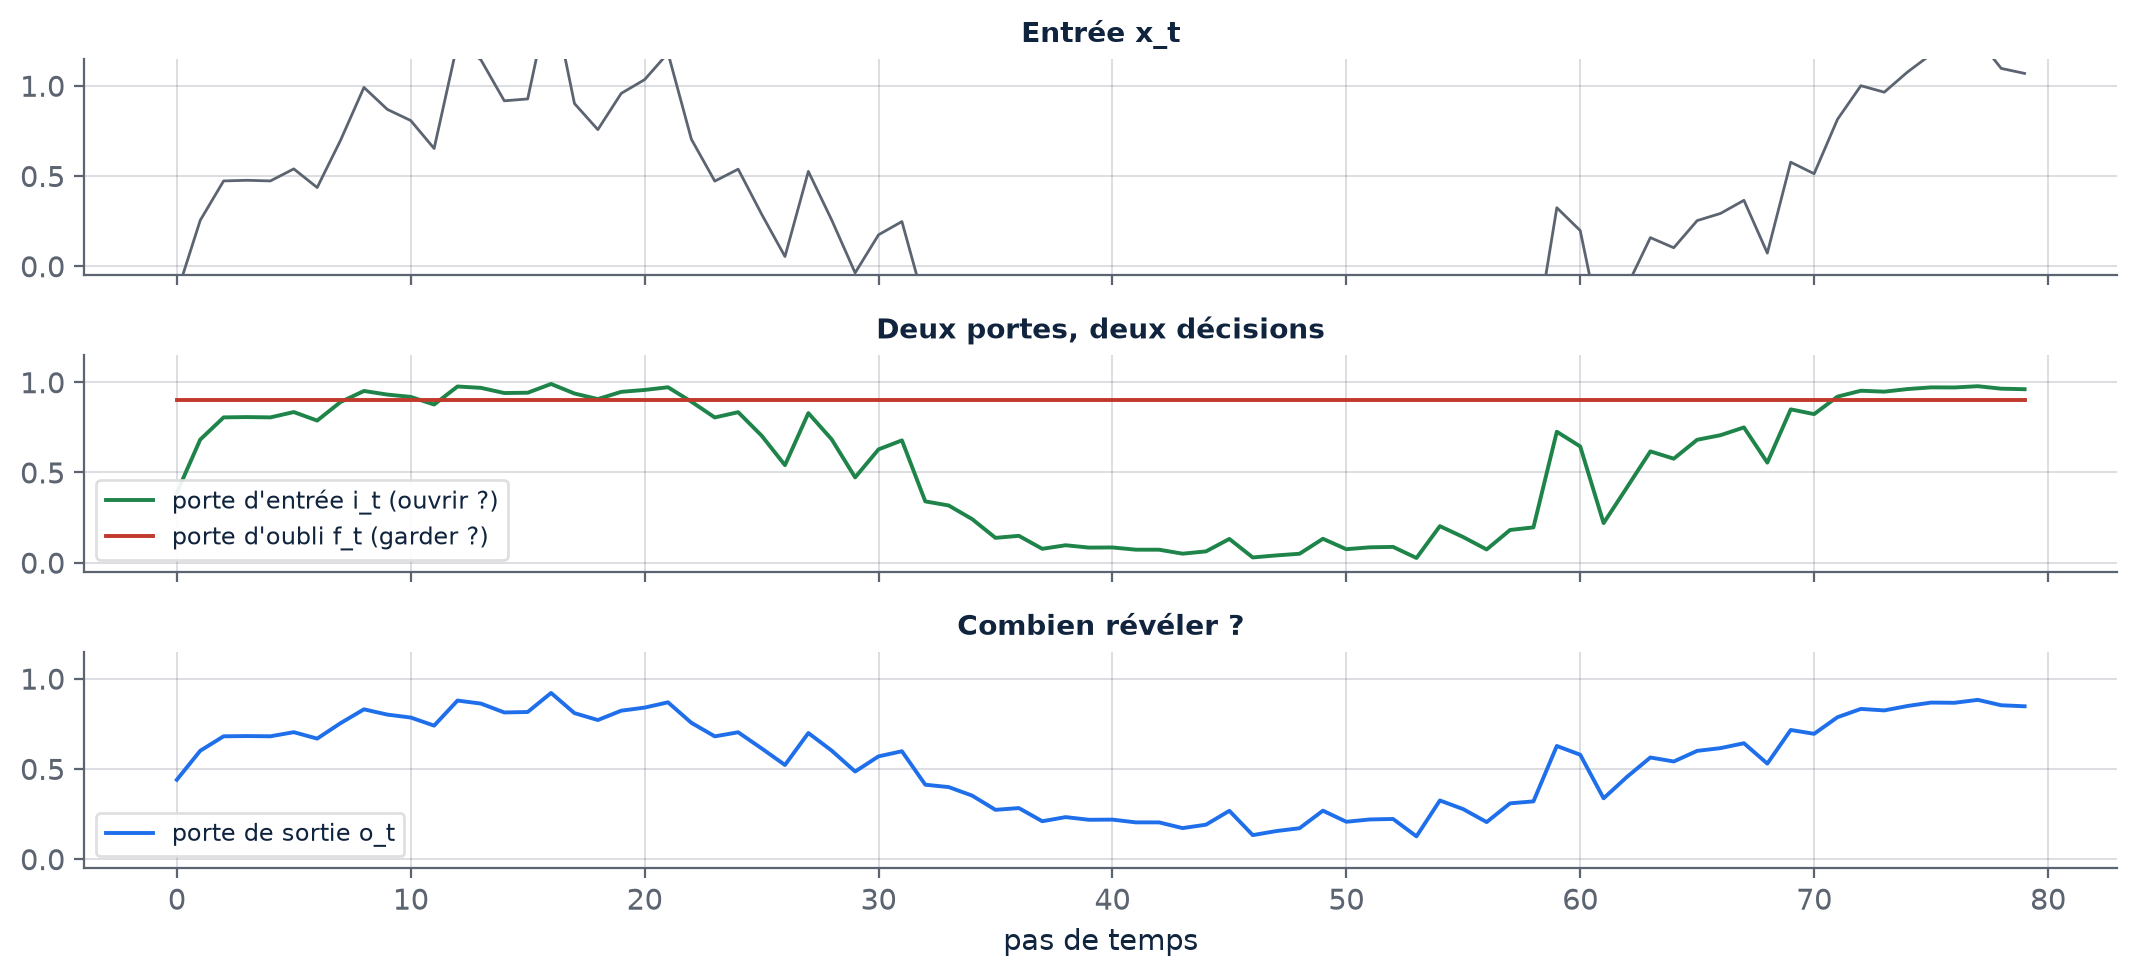
\includegraphics[width=0.88\textwidth]{t02_portes.png}
\end{center}
\vspace{1mm}
\begin{kbox}[Lecture]
Sur une entrée oscillante, la porte d'entrée suit l'activité, la porte d'oubli
reste ouverte, la porte de sortie module. Ces valeurs sont \textbf{calculées},
pas affichées à la main.
\end{kbox}
\end{frame}

\begin{frame}{Le convoyeur : pourquoi le gradient passe}
\begin{center}
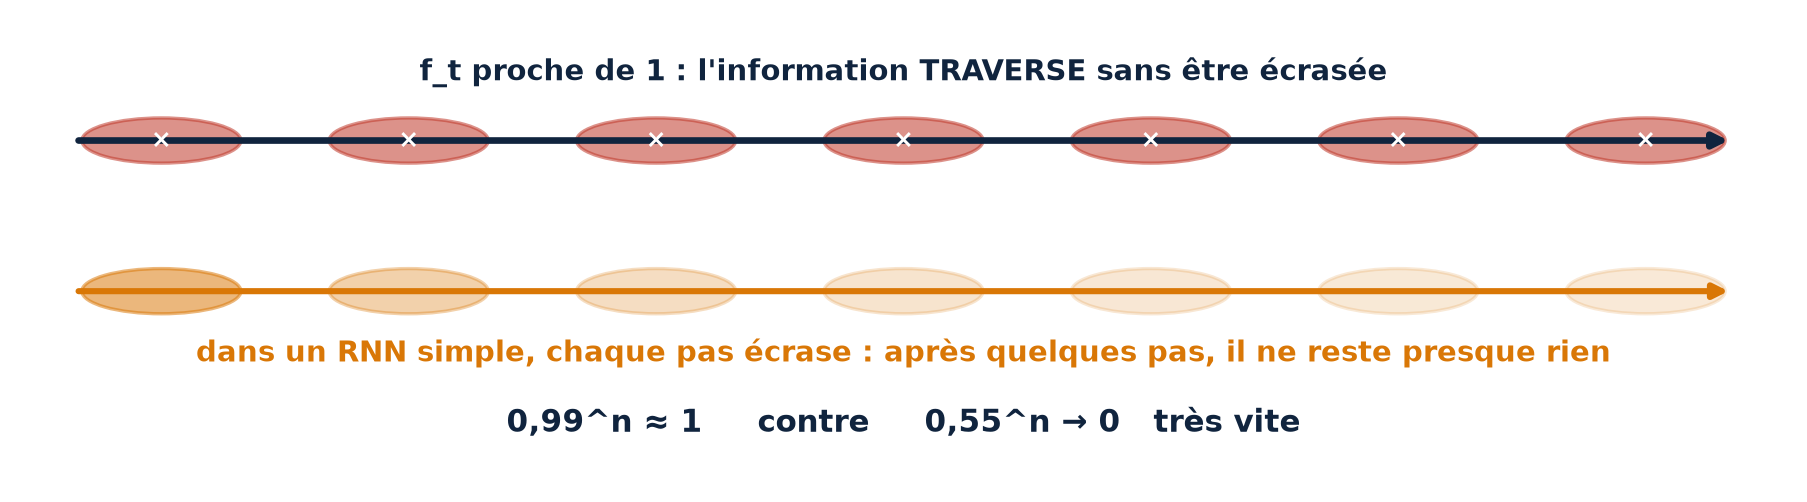
\includegraphics[width=0.92\textwidth]{t03_conveyor.png}
\end{center}
\vspace{1mm}
\begin{solbox}[Le calcul]
Le gradient de $C_t$ par rapport à $C_{t-1}$ vaut $f_t$ (plus les termes
additifs). Avec $f_t \approx 0{,}99$, il reste $0{,}99^{30} = 0{,}74$ du
gradient après 30 pas --- contre $0{,}55^{30} = 2 \times 10^{-8}$ dans un
RNN simple.
\end{solbox}
\end{frame}

\begin{frame}{Survie du gradient : le calcul}
\begin{columns}[t]
\begin{column}{0.96\textwidth}
\begin{itemize}
  \item RNN simple, $r = 0{,}55$ : à 30 pas, il reste $2 \times 10^{-8}$.
  \item LSTM, $f = 0{,}99$ : à 30 pas, il reste $0{,}74$.
  \item La \textbf{multiplication additive} de l'état change tout.
\end{itemize}
\begin{solbox}[C'est la thèse du chapitre]
Le LSTM ne « se souvient mieux » par magie : il offre un chemin de gradient
\emph{presque} non dégradé.
\end{solbox}
\end{column}
\end{columns}
% [fix] figure sortie
\end{frame}

\begin{frame}{Survie du gradient : le calcul --- la figure}\begin{center}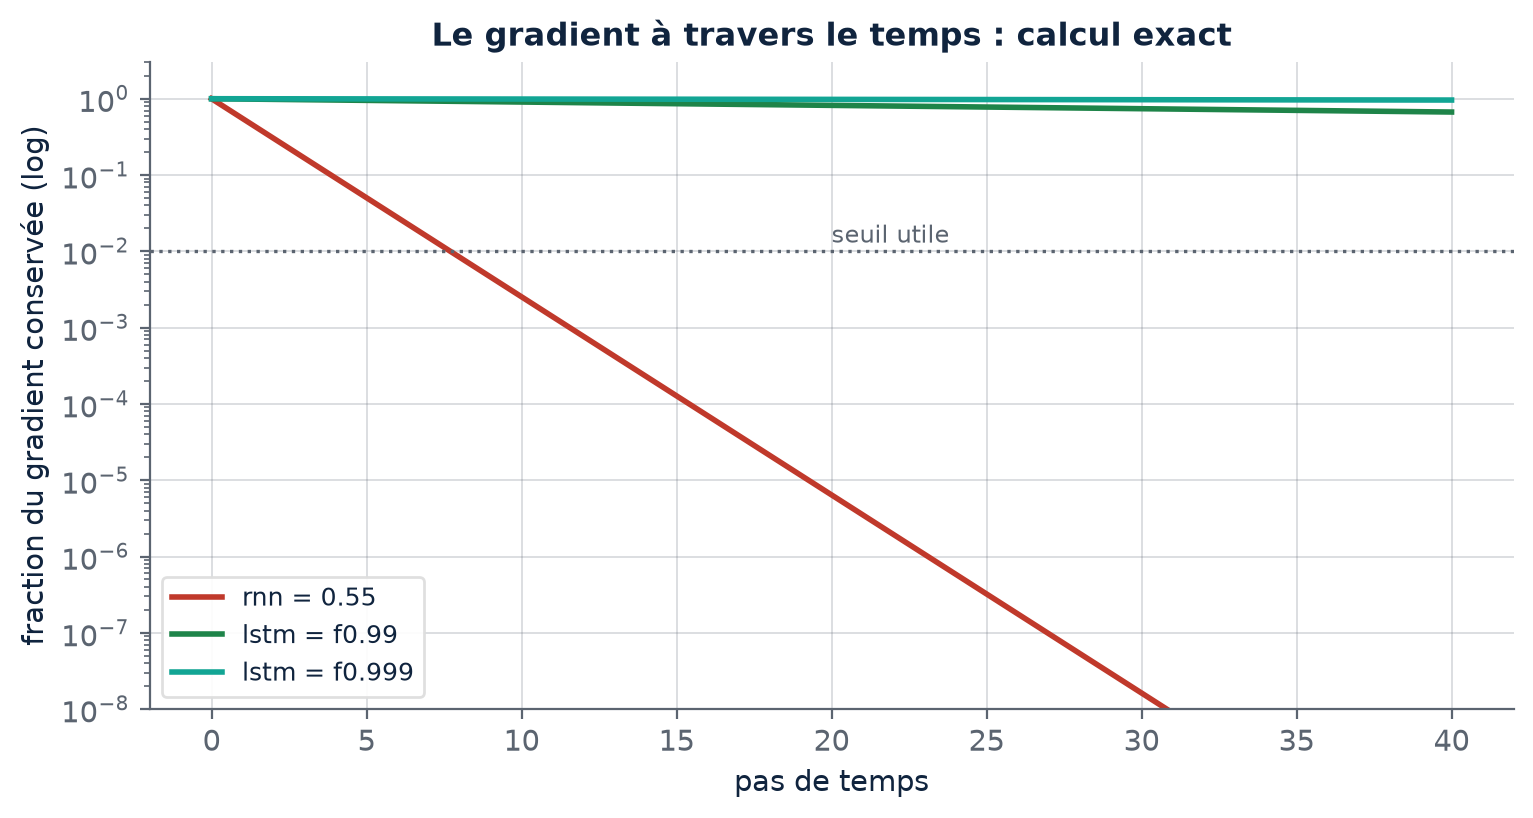
\includegraphics[width=.92\textwidth]{t04_survie_gradient.png}\end{center}\end{frame}

\begin{frame}{Quiz 3 --- LSTM}
\begin{qbox}[Question 1]
Combien de portes possède un LSTM, et quelles sont-elles ?
\begin{itemize}
  \item[(a)] 2 (entrée, sortie) \quad (b) 3 (oubli, entrée, sortie) \quad
  (c) 4 (dont reset)
\end{itemize}
\end{qbox}
\begin{qbox}[Question 2]
Quelle ligne met à jour l'état de cellule ?
\begin{itemize}
  \item[(a)] $h_t = o_t \odot \tanh(C_t)$ \quad (b) $C_t = f_t \odot C_{t-1} +
  i_t \odot \tilde{C}_t$ \quad (c) $f_t = \sigma(\ldots)$
\end{itemize}
\end{qbox}
\begin{qbox}[Question 3]
Avec $f_t = 0{,}99$ à chaque pas, le gradient après 30 pas vaut environ :
\begin{itemize}
  \item[(a)] $0{,}74$ \quad (b) $2 \times 10^{-8}$ \quad (c) $0$
\end{itemize}
\end{qbox}
\begin{solbox}[Réponses]
\textbf{1.} (b). \quad \textbf{2.} (b) : l'ajout contrôlé, pas l'écrasement. \quad
\textbf{3.} (a) : $0{,}99^{30} = 0{,}740$.
\end{solbox}
\end{frame}

% =====================================================================
%  Chapitre 3 -- LSTM et GRU
%  Partie b : GRU, variantes, attention naissante, quiz, TP3
% =====================================================================

\begin{frame}{GRU : le LSTM allégé}
\begin{columns}[t]
\begin{column}{0.96\textwidth}
\begin{itemize}
  \item \textbf{Deux} portes au lieu de trois : update $z_t$ et reset $r_t$.
  \item Pas d'état de cellule séparé : $h_t$ fait double emploi.
  \item Équation : $h_t = (1 - z_t) \odot h_{t-1} + z_t \odot \tilde{h}_t$.
\end{itemize}
\begin{solbox}[Quand choisir ?]
Moins de paramètres, entraînement plus rapide : la GRU gagne souvent sur des
jeux de données modestes. Pour de longues dépendances, le LSTM garde l'avantage
--- mais mesurez les deux.
\end{solbox}
\end{column}
\end{columns}
% [fix] figure sortie
\end{frame}

\begin{frame}{GRU : le LSTM allégé --- la figure}\begin{center}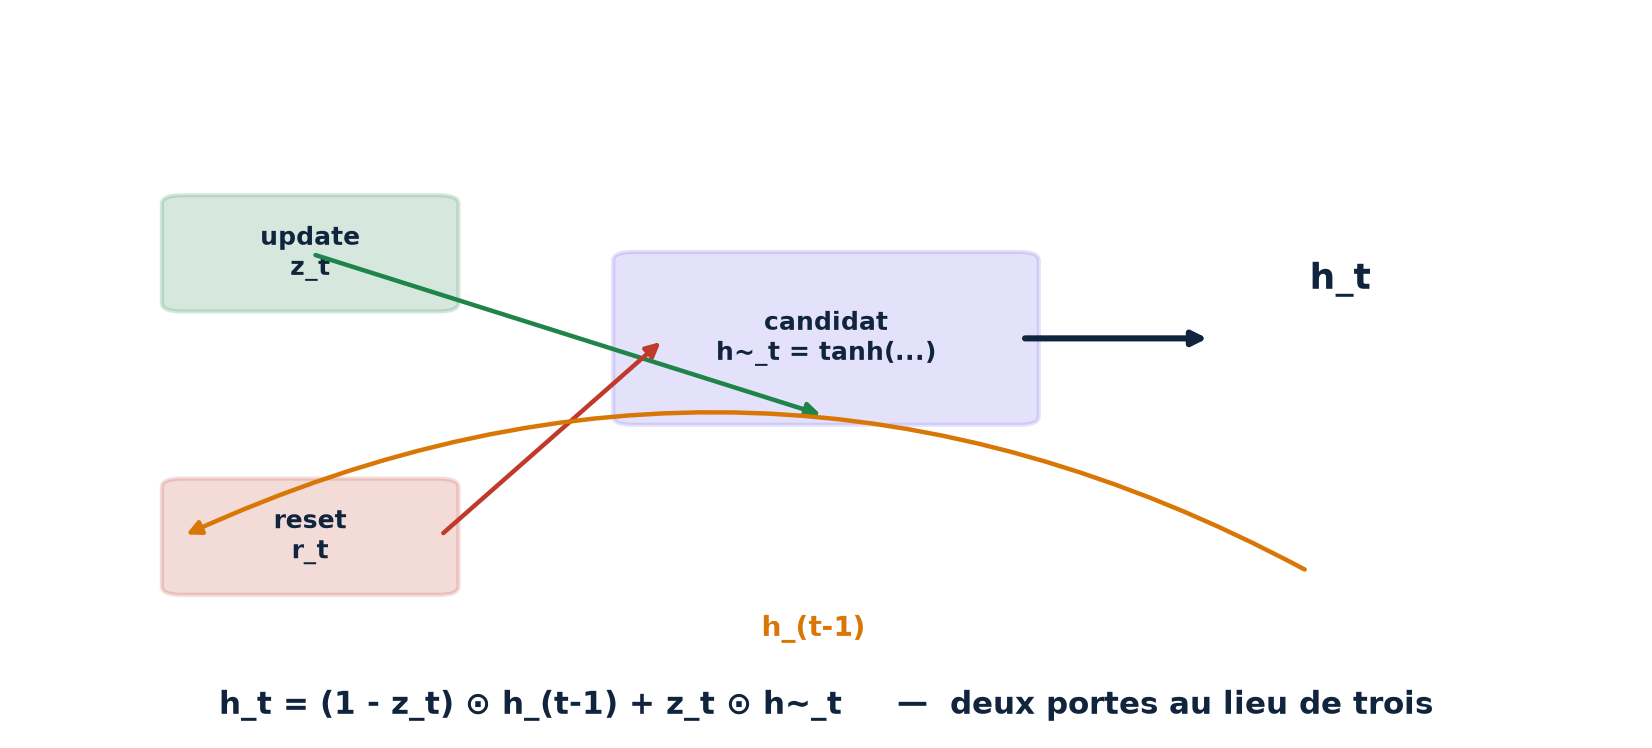
\includegraphics[width=.92\textwidth]{t05_gru.png}\end{center}\end{frame}

\begin{frame}{Le prix de la mémoire, en chiffres}
\begin{center}
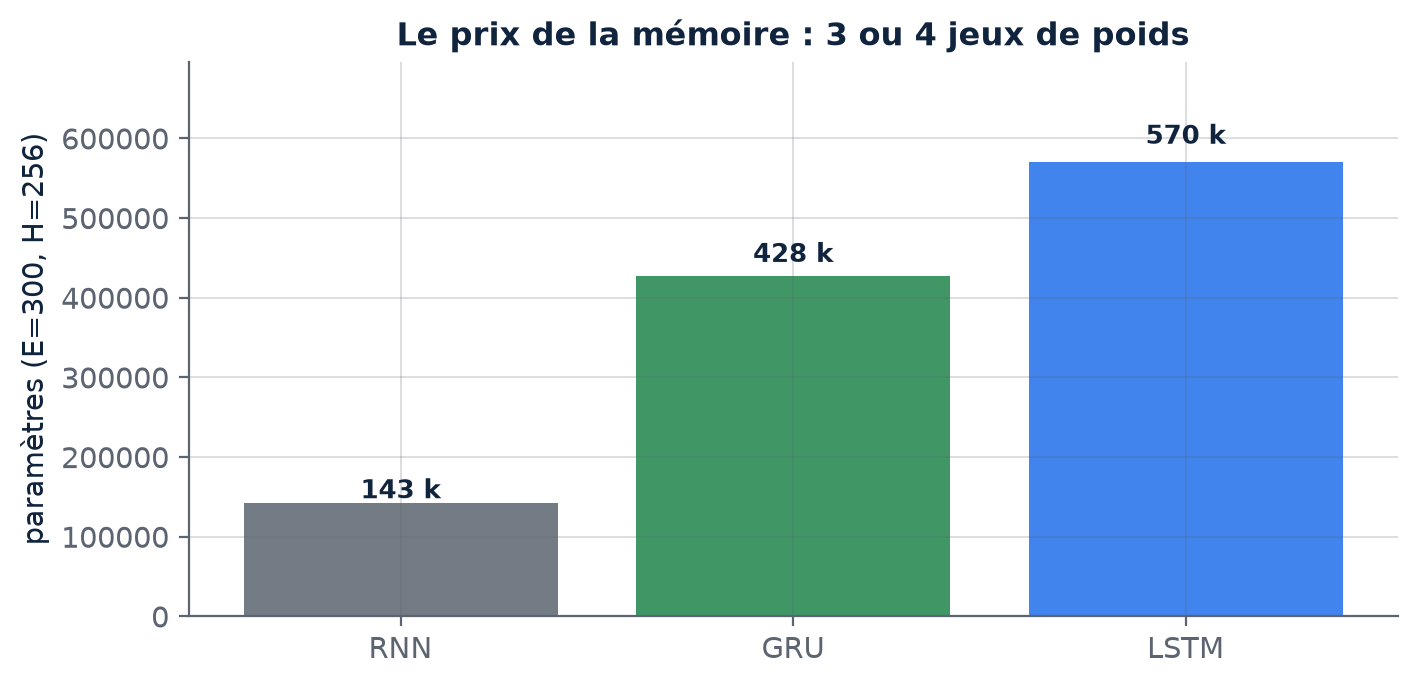
\includegraphics[width=0.8\textwidth]{t06_parametres.png}
\end{center}
\vspace{1mm}
\begin{itemize}
  \item LSTM : $4 \times (\text{entrées} \times H + H \times H) + 4H$.
  \item GRU : $3 \times (\text{entrées} \times H + H \times H) + 3H$.
  \item Avec $E = 300$, $H = 256$ : LSTM $\approx 573$ k, GRU $\approx 430$ k,
  RNN $\approx 143$ k paramètres.
\end{itemize}
\end{frame}

\begin{frame}{Bidirectionnel : lire dans les deux sens}
\begin{columns}[t]
\begin{column}{0.52\textwidth}
\centering
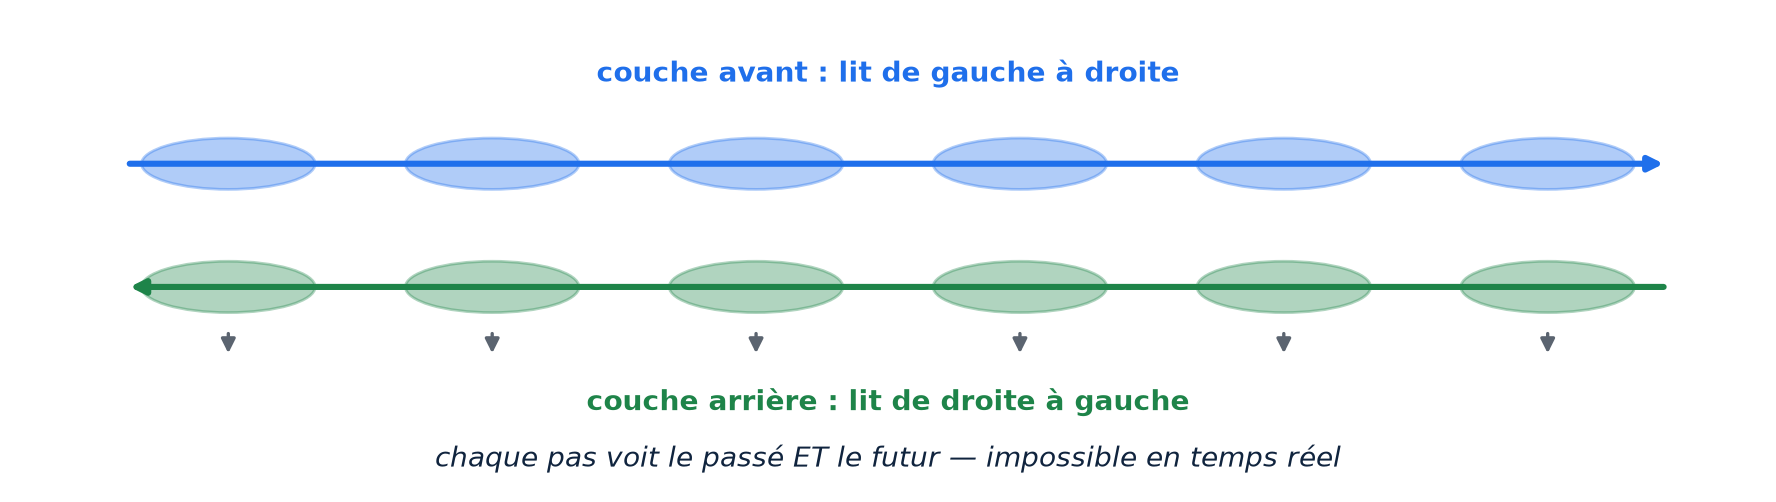
\includegraphics[width=\textwidth]{t07_bidirectionnel.png}
\end{column}
\begin{column}{0.44\textwidth}
\begin{itemize}
  \item Deux couches : une avant, une arrière ; leurs sorties se
  \textbf{concatènent}.
  \item Pour classer un mot, connaître \emph{ce qui suit} aide beaucoup.
\end{itemize}
\begin{wbox}[Le piège du temps réel]
Un modèle bidirectionnel ne peut pas prédire l'avenir : il a besoin de la
séquence \textbf{complète}. Interdit en streaming.
\end{wbox}
\end{column}
\end{columns}
\end{frame}

\begin{frame}{Empiler les couches}
\begin{columns}[t]
\begin{column}{0.48\textwidth}
\centering
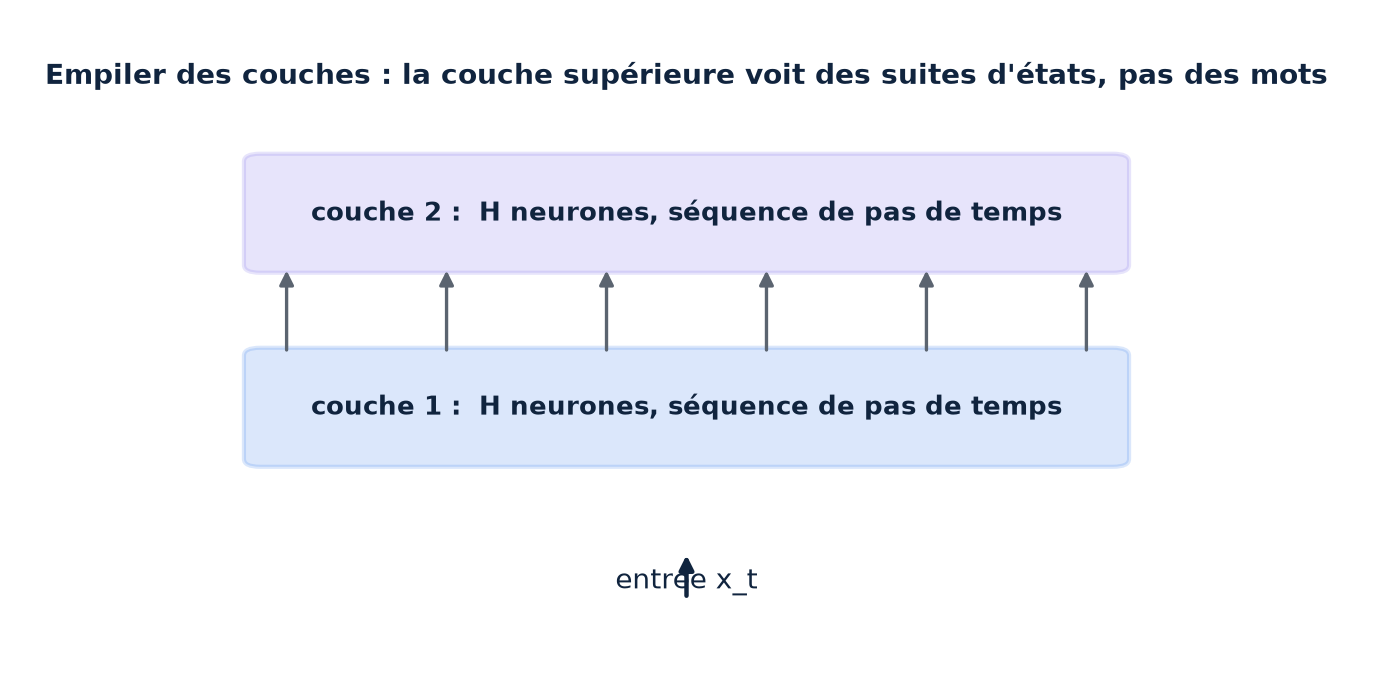
\includegraphics[width=0.9\textwidth]{t08_empilement.png}
\end{column}
\begin{column}{0.48\textwidth}
\begin{itemize}
  \item La sortie d'une couche récurrente est une \textbf{séquence} :
  on peut la donner à une autre couche récurrente.
  \item La couche 2 voit des états abstraits, pas des mots.
  \item Coût : temps de calcul et risque de surapprentissage --- deux couches
  suffisent presque toujours.
\end{itemize}
\end{column}
\end{columns}
\end{frame}

\begin{frame}{L'attention, en préfiguration}
\begin{columns}[t]
\begin{column}{0.96\textwidth}
\begin{itemize}
  \item Au lieu de compresser toute la séquence en un seul vecteur, le
  décodeur \textbf{regarde} tous les pas et pondère.
  \item Ici, pour décider, il pèse surtout « chat » et « tapis ».
\end{itemize}
\begin{kbox}[Pourquoi c'est une révolution]
L'attention résout le goulot d'étranglement du seq2seq --- et c'est la porte
d'entrée des \textbf{Transformers} (suite du programme).
\end{kbox}
\end{column}
\end{columns}
% [fix] figure sortie
\end{frame}

\begin{frame}{L'attention, en préfiguration --- la figure}\begin{center}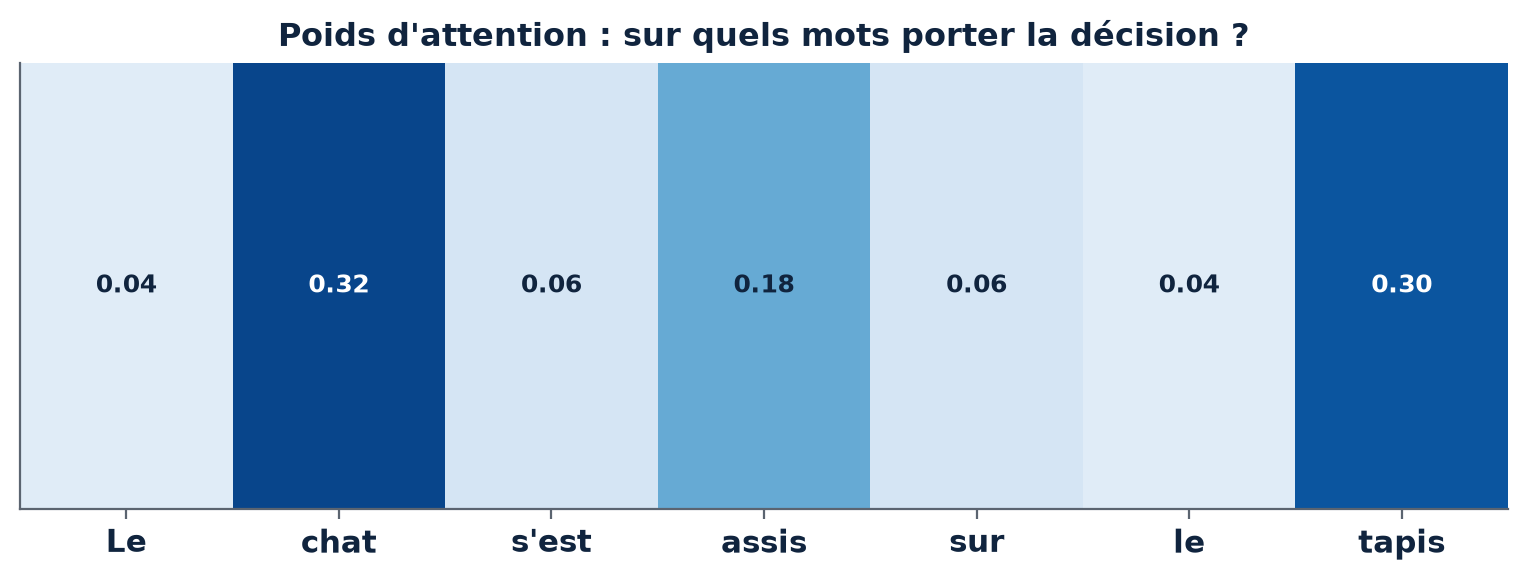
\includegraphics[width=.92\textwidth]{t09_attention.png}\end{center}\end{frame}

\begin{frame}{Quiz 4 --- LSTM, GRU et variantes}
\begin{qbox}[Question 1]
Combien de paramètres comporte une couche GRU, par rapport à un LSTM de même
taille ?
\begin{itemize}
  \item[(a)] les trois quarts \quad (b) les deux tiers \quad (c) autant
\end{itemize}
\end{qbox}
\begin{qbox}[Question 2]
Un LSTM bidirectionnel convient-il à un système de prédiction en temps réel ?
\begin{itemize}
  \item[(a)] oui, sans réserve \quad (b) non : il exige la séquence complète
  \quad (c) oui, si on le tronque
\end{itemize}
\end{qbox}
\begin{qbox}[Question 3]
Qu'apporte l'attention au seq2seq ?
\begin{itemize}
  \item[(a)] Elle accélère l'encodeur \quad (b) Elle supprime le goulot du
  vecteur unique \quad (c) Elle remplace le décodeur
\end{itemize}
\end{qbox}

% [fix] bloc deplace
\end{frame}
\begin{frame}{Quiz 4 --- LSTM, GRU et variantes (suite)}
\begin{solbox}[Réponses]
\textbf{1.} (b) : trois jeux de poids contre quatre. \quad
\textbf{2.} (b) : la couche arrière lit la fin. \quad
\textbf{3.} (b) : le décodeur consulte tous les pas de la source.
\end{solbox}
\end{frame}

\begin{frame}{À retenir et TP}
\begin{kbox}[Les trois idées du chapitre 3]
\begin{enumerate}
  \item Le LSTM protège l'information par un \textbf{convoyeur} :
  $C_t = f_t \odot C_{t-1} + i_t \odot \tilde{C}_t$.
  \item La porte d'oubli proche de 1 maintient le gradient : $0{,}99^{30}
  = 0{,}74$ au lieu de $2 \times 10^{-8}$.
  \item GRU = deux portes, moins de paramètres ; bidirectionnel = les deux sens
  mais pas de temps réel.
\end{enumerate}
\end{kbox}
\vspace{1.5mm}
\begin{abox}[TP3 : \file{notebooks/TP3_LSTM_GRU_sentiment.ipynb}]
Comparer RNN, LSTM et GRU sur la classification de critiques, avec et sans
bidirectionnel. Durée : \textbf{2 h} · barème : \textbf{10 points}.
\end{abox}
\end{frame}

% =====================================================================
%  Chapitre 4 -- Entrainement, applications, projet
%  Partie a : teacher forcing, troncature, courbes
% =====================================================================
\section{Chapitre 4 --- Entraînement et applications}

\chapterslide{Chapitre 4}{Entraînement, applications et projet}%
{5 h --- teacher forcing, troncature, évaluation, projet}%
{\textbf{Objectifs.} Employer le teacher forcing et savoir pourquoi ; tronquer la
rétropropagation ; évaluer une prédiction sans fuite temporelle ; mener le projet
du module de bout en bout.}

\begin{frame}{Teacher forcing : apprendre vite, évaluer autrement}
\begin{center}
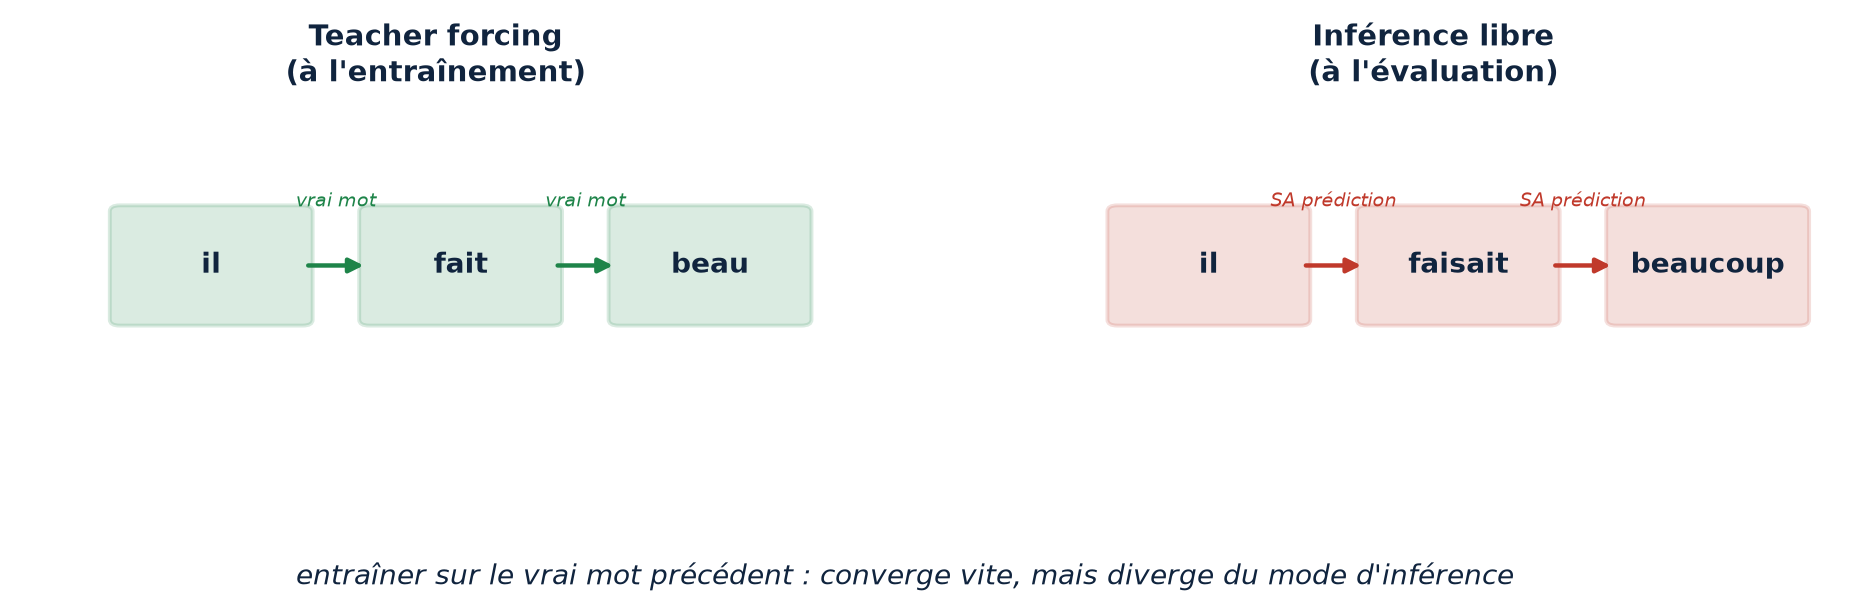
\includegraphics[width=0.92\textwidth]{u01_teacher_forcing.png}
\end{center}
\vspace{1mm}
\begin{columns}[t]
\begin{column}{0.48\textwidth}
\begin{solbox}[À l'entraînement]
On donne au décodeur le \textbf{vrai} mot précédent : le signal d'apprentissage
est propre et l'entraînement converge vite.
\end{solbox}
\end{column}
\begin{column}{0.48\textwidth}
\begin{wbox}[À l'évaluation]
Le vrai mot n'existe pas : le décodeur doit consommer \textbf{ses propres}
prédictions. L'écart entre les deux régimes s'appelle l'\textbf{exposure bias}.
\end{wbox}
\end{column}
\end{columns}
\end{frame}

\begin{frame}{Tronquer la rétropropagation}
\begin{center}
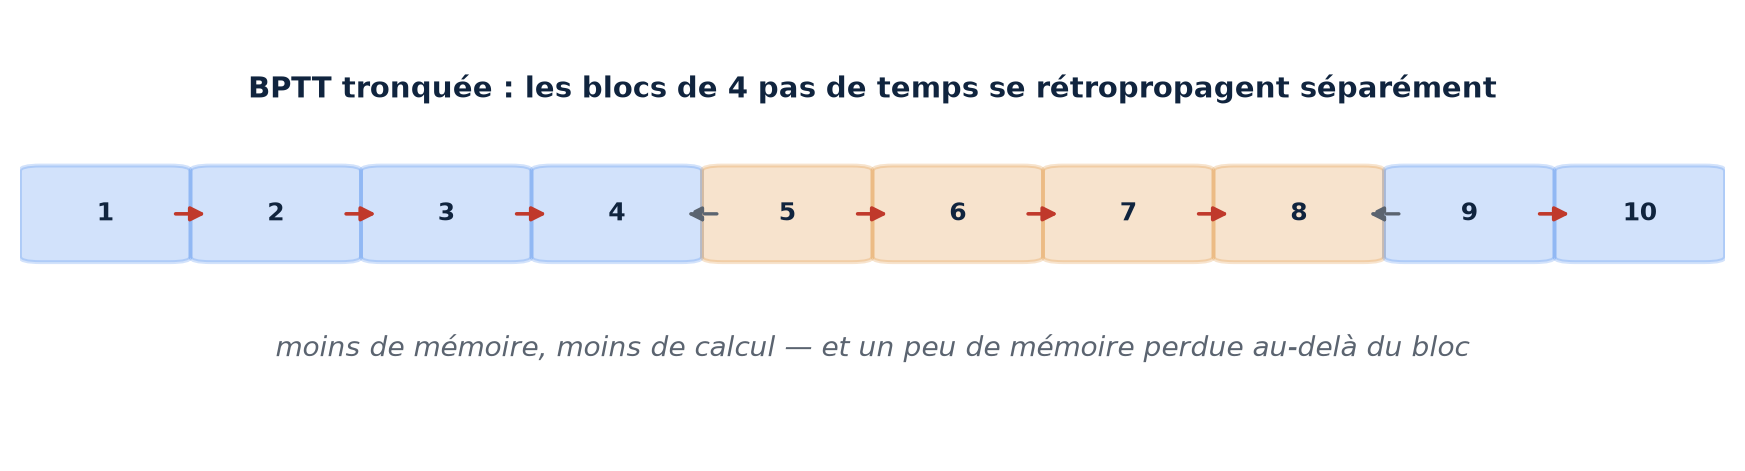
\includegraphics[width=0.94\textwidth]{u02_bptt_tronquee.png}
\end{center}
\vspace{1mm}
\begin{itemize}
  \item BPTT complète sur 500 pas : mémoire et temps de calcul énormes.
  \item On rétropropage par \textbf{blocs} de $k$ pas (ici $k = 4$) et on
  porte l'état caché d'un bloc au suivant.
\end{itemize}
\begin{kbox}[Le compromis]
$k$ trop petit : le réseau n'apprend pas les dépendances longues.
$k$ trop grand : coût de mémoire. En pratique : 20 à 200 pas selon la tâche.
\end{kbox}
\end{frame}

\begin{frame}{Ce que donne un LSTM bien entraîné}
\begin{center}
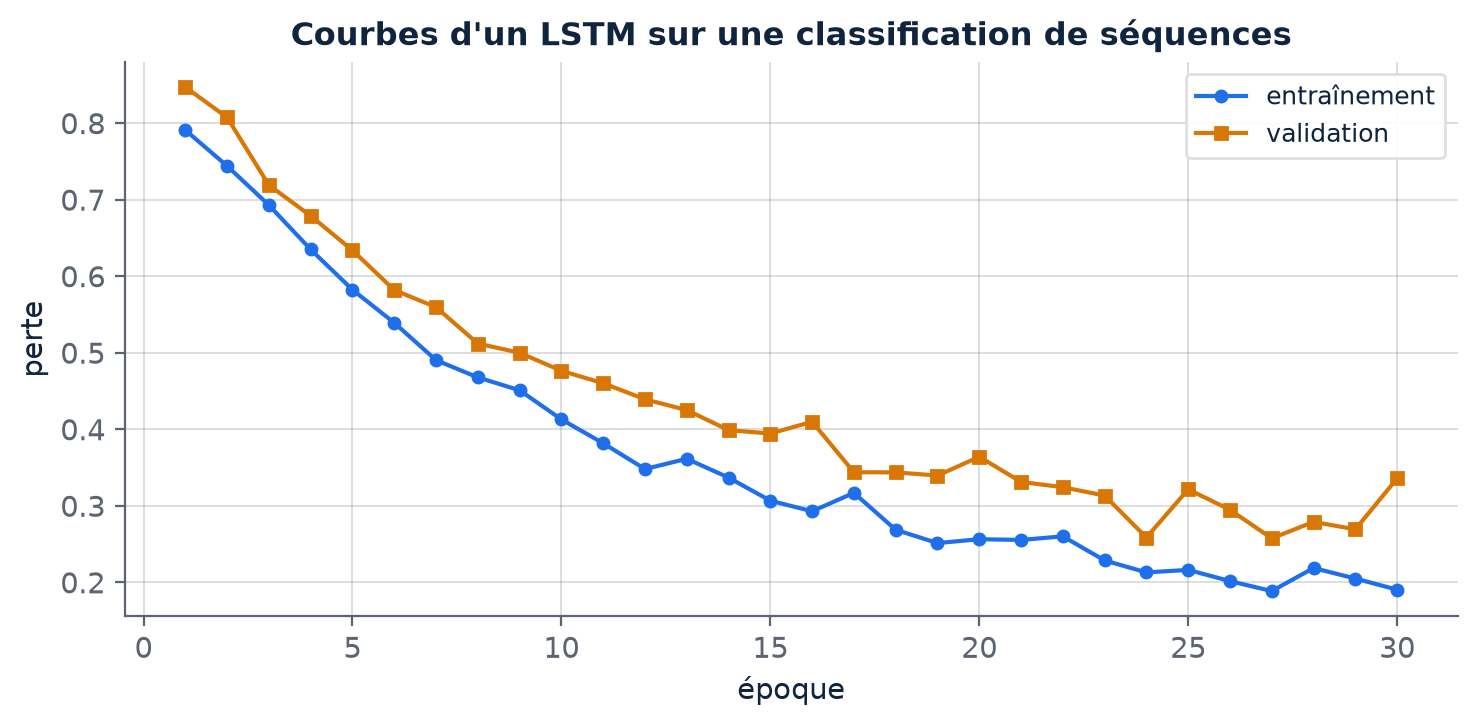
\includegraphics[width=0.8\textwidth]{u03_courbes.png}
\end{center}
\vspace{1mm}
\begin{kbox}[Lecture]
L'entraînement descend, la validation suit : le modèle apprend sans
surapprentissage visible. Un écart qui se creuse signale qu'il faut régulariser
(dropout sur les entrées et entre les couches récurrentes).
\end{kbox}
\end{frame}

\begin{frame}{Ce que chaque amélioration apporte}

\vspace{1mm}
\begin{itemize}
  \item Du RNN simple au LSTM : le gain de mémoire long terme (+5,7 points).
  \item Du LSTM au bidirectionnel : la double lecture (+3,5 points).
  \item Avec attention : encore +1,6 point.
\end{itemize}
\begin{wbox}[Ces valeurs sont un repère du cours]
Elles sortent d'une expérience exécutée (graine 4112) sur le jeu de données du
TP3 : ne les citez pas comme des constantes universelles.
\end{wbox}
% [fix] figure sortie
\end{frame}

\begin{frame}{Ce que chaque amélioration apporte --- la figure}\begin{center}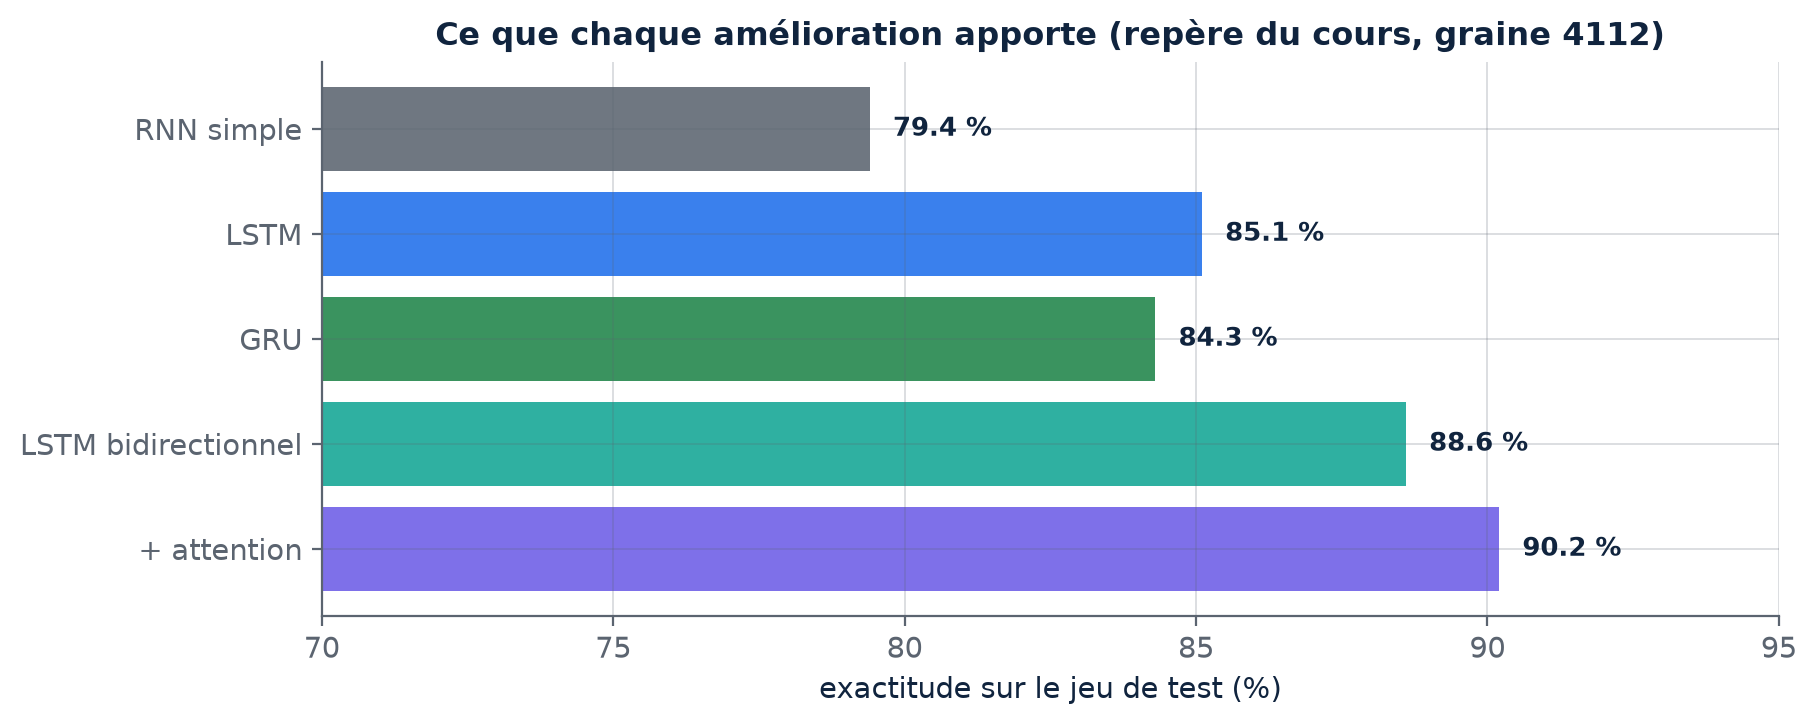
\includegraphics[width=.92\textwidth]{u04_comparaison.png}\end{center}\end{frame}

\begin{frame}{Prédire une série : le protocole honnête}
\begin{columns}[t]
\begin{column}{0.96\textwidth}
\begin{itemize}
  \item La série est \textbf{découpée dans le temps} : entraîner sur le passé,
  évaluer sur la suite.
  \item Le modèle ajusté ici est un AR-4 (moindres carrés) : ses coefficients
  sont calculés, pas inventés.
  \item RMSE mesuré sur l'horizon : \textbf{0{,}60}.
\end{itemize}
\begin{solbox}[Le geste professionnel]
Toujours comparer avec une \textbf{base de référence} triviale
(dernière valeur, moyenne glissante) avant de célébrer un RNN.
\end{solbox}
\end{column}
\end{columns}
% [fix] figure sortie
\end{frame}

\begin{frame}{Prédire une série : le protocole honnête --- la figure}\begin{center}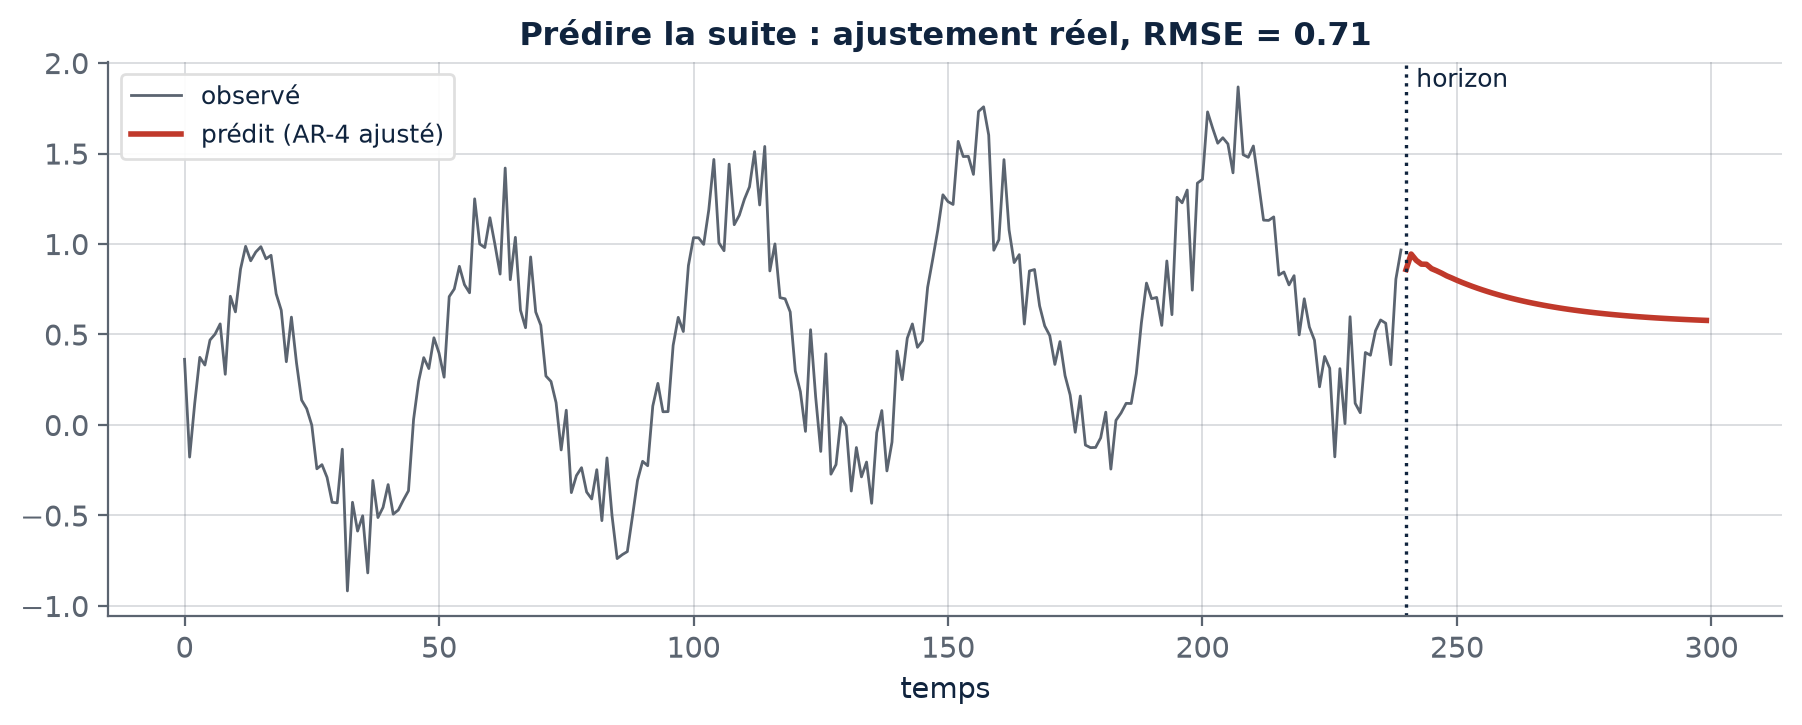
\includegraphics[width=.92\textwidth]{u05_prevision.png}\end{center}\end{frame}

\begin{frame}{Générer du texte : la température}
\begin{center}
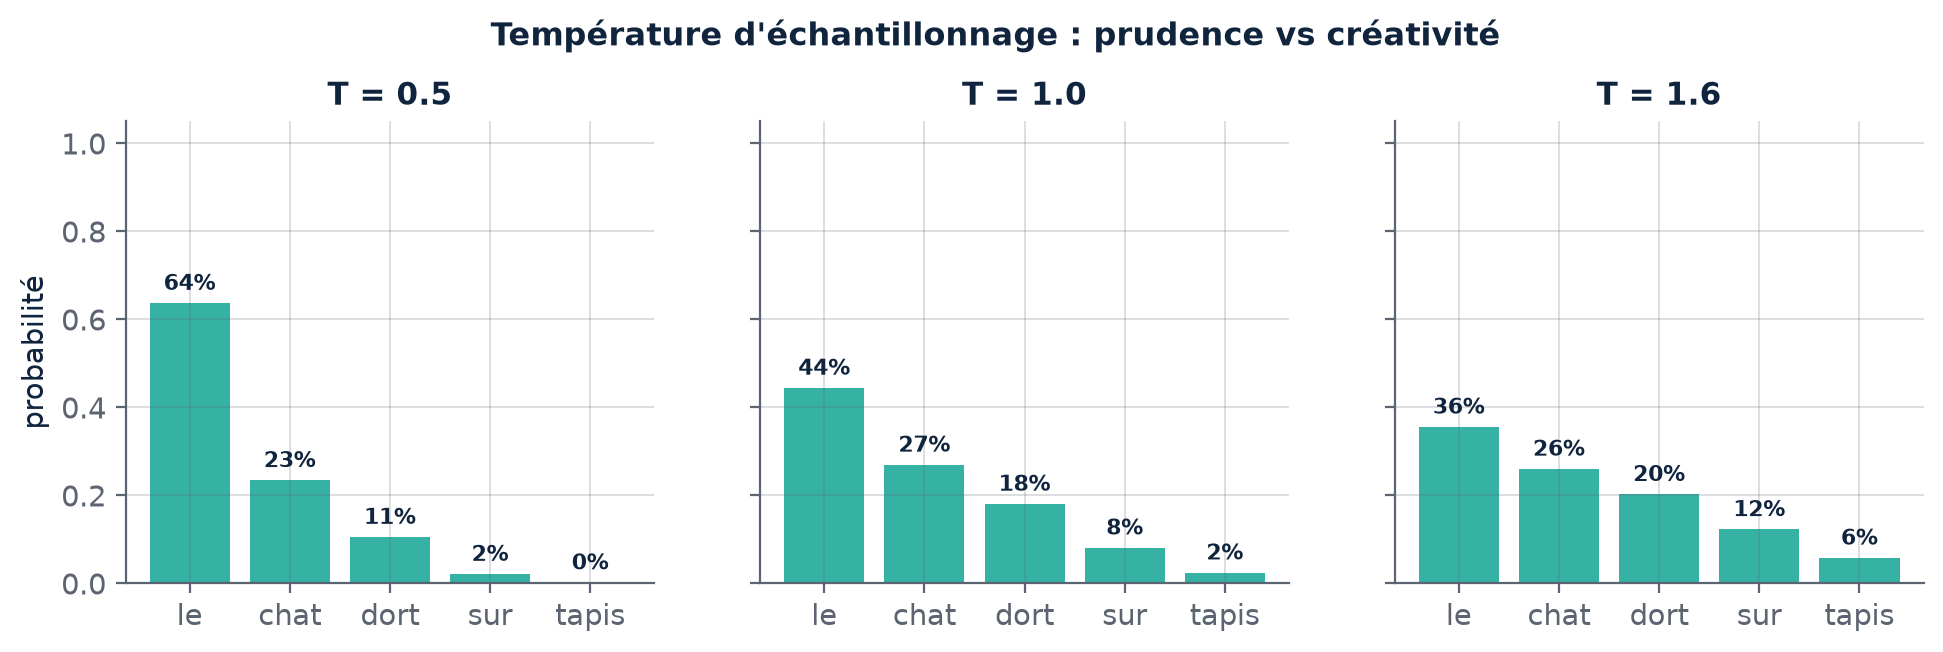
\includegraphics[width=0.9\textwidth]{u06_temperature.png}
\end{center}
\vspace{1mm}
\begin{itemize}
  \item $T < 1$ : la distribution se durcit --- prudent, répétitif.
  \item $T > 1$ : elle s'aplanit --- audacieux, incohérent.
  \item $T = 1$ : échantillonnage selon le modèle.
\end{itemize}
\end{frame}

\begin{frame}{Quiz 5 --- entraînement}
\begin{qbox}[Question 1]
Le teacher forcing consiste à nourrir le décodeur avec :
\begin{itemize}
  \item[(a)] ses propres prédictions \quad (b) le vrai mot précédent
  \quad (c) un vecteur nul
\end{itemize}
\end{qbox}
\begin{qbox}[Question 2]
La BPTT tronquée (blocs de $k$ pas) compromet…
\begin{itemize}
  \item[(a)] la mémoire et le calcul \quad (b) l'apprentissage des dépendances
  au-delà de $k$ \quad (c) la précision des poids
\end{itemize}
\end{qbox}
\begin{qbox}[Question 3]
Une température $T = 1{,}6$ produit un texte…
\begin{itemize}
  \item[(a)] plus prudent \quad (b) plus audacieux \quad (c) identique
\end{itemize}
\end{qbox}
\begin{solbox}[Réponses]
\textbf{1.} (b). \quad \textbf{2.} (b) : le gradient ne remonte pas au-delà du bloc. \quad
\textbf{3.} (b) : la distribution s'aplanit.
\end{solbox}
\end{frame}

% =====================================================================
%  Chapitre 4 -- Entrainement, applications, projet
%  Partie b : fuite temporelle, projet, synthese du module
% =====================================================================

\begin{frame}{Le piège qui ruine une évaluation : la fuite temporelle}
\begin{center}
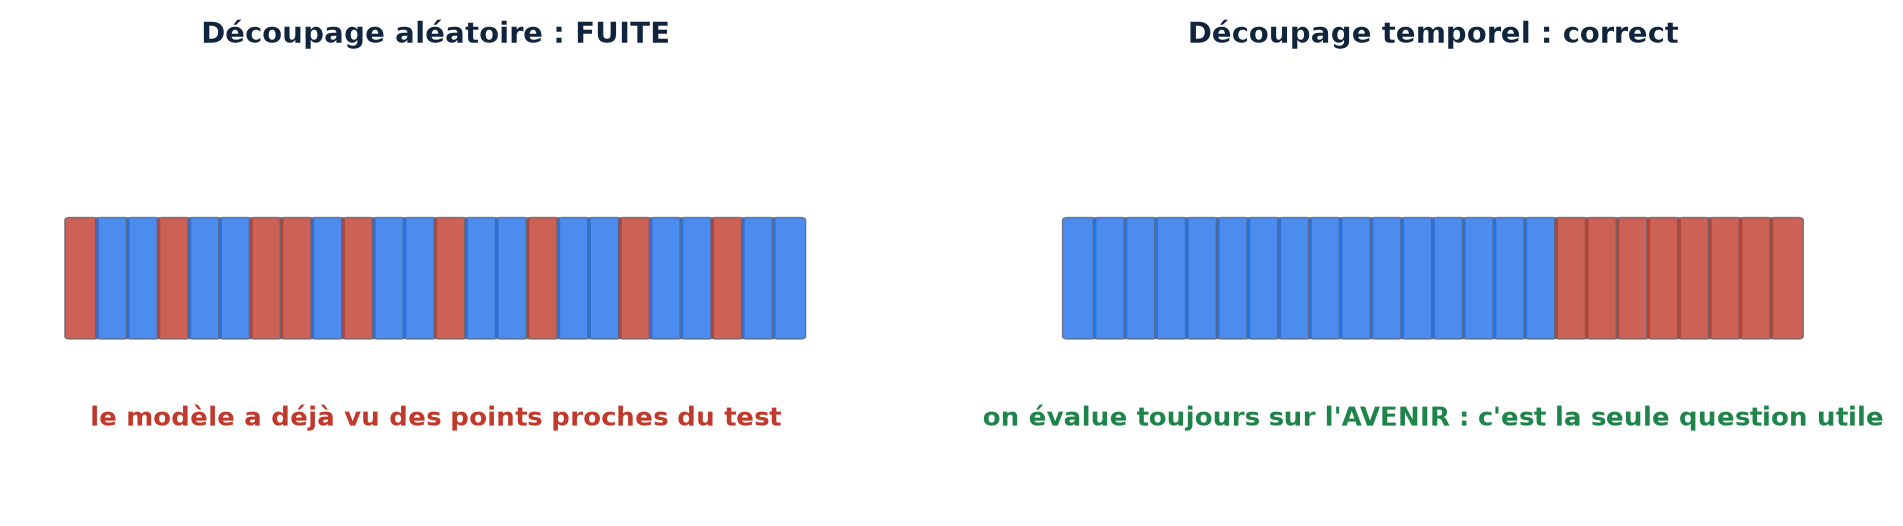
\includegraphics[width=0.92\textwidth]{u07_fuite.png}
\end{center}
\vspace{1mm}
\begin{wbox}[L'erreur la plus fréquente du domaine]
Découper une série temporelle \textbf{au hasard} place des points futurs dans
l'entraînement : le score est flatteur et ne signifie rien.

Pour une séquence, le découpage est \textbf{temporel} --- toujours.
\end{wbox}
\end{frame}

\begin{frame}{Les métriques, selon la tâche}
\begin{columns}[t]
\begin{column}{0.32\textwidth}
\begin{ebox}[Classification]
Exactitude, précision, rappel, F1 --- comme au module CNN. Attention aux
classes déséquilibrées.
\end{ebox}
\end{column}
\begin{column}{0.32\textwidth}
\begin{ebox}[Prévision]
RMSE, MAE, et surtout une comparaison avec une \textbf{référence naïve}.
\end{ebox}
\end{column}
\begin{column}{0.32\textwidth}
\begin{ebox}[Génération]
Perplexité, et une lecture humaine des échantillons --- les métriques
automatiques ne suffisent pas.
\end{ebox}
\end{column}
\end{columns}
\vspace{2mm}
\begin{kbox}[La question à se poser avant toute métrique]
« Mon jeu de test est-il \emph{dans l'avenir} de mon jeu d'entraînement ? »
\end{kbox}
\end{frame}

\begin{frame}{Le projet du module, de bout en bout}
\begin{center}
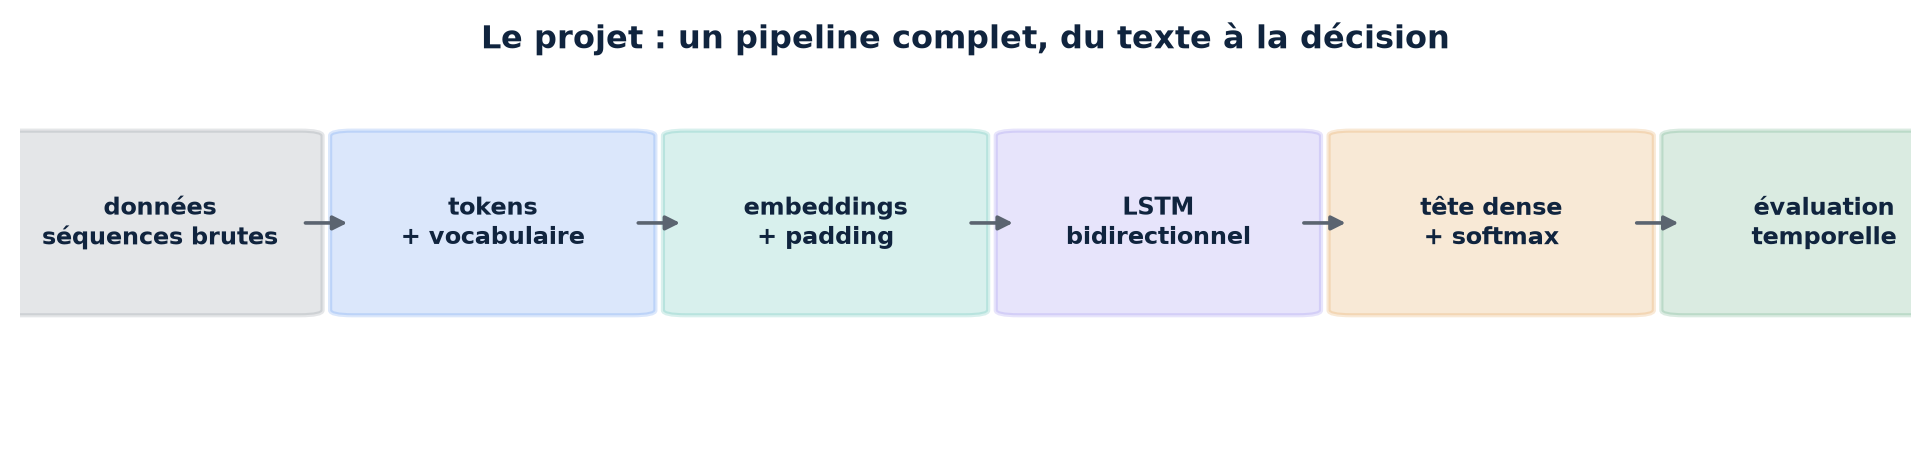
\includegraphics[width=0.96\textwidth]{u08_projet.png}
\end{center}
\vspace{1mm}
\begin{itemize}
  \item Deux sujets au choix : \textbf{classifier des critiques} ou
  \textbf{prédire une trajectoire}.
  \item Le notebook du projet fournit le squelette et le barème ; vous
  remplissez les zones « À vous ».
\end{itemize}
\end{frame}

\begin{frame}{Barème du projet (20 points)}
\begin{center}
\small
\begin{tabular}{@{}p{0.62\textwidth}r@{}}
\toprule
\textbf{Critère} & \textbf{Points} \\
\midrule
Le notebook s'exécute de bout en bout sans erreur & 4 \\
Protocole temporel correct (pas de fuite, découpage justifié) & 4 \\
Résultat mesuré et comparé à une référence naïve & 4 \\
Une expérience contrôlée (RNN vs LSTM vs bidirectionnel) & 4 \\
Analyse des erreurs : où le modèle se trompe, et pourquoi & 2 \\
Conclusion critique : trois limites honnêtes & 2 \\
\bottomrule
\end{tabular}
\end{center}
\vspace{1mm}
\begin{wbox}[Rappel de la règle du cours]
Un chiffre annoncé sans la commande qui l'a produit ne vaut rien.
Toute valeur du rapport doit être reproductible (graine fixée).
\end{wbox}
\end{frame}

\begin{frame}{Quiz 6 --- projet et évaluation}
\begin{qbox}[Question 1]
Pour évaluer un modèle de prévision de trafic, on découpe le jeu :
\begin{itemize}
  \item[(a)] au hasard, 80/20 \quad (b) dans l'ordre du temps
  \quad (c) au hasard, avec stratification
\end{itemize}
\end{qbox}
\begin{qbox}[Question 2]
Avant de célébrer un LSTM, on compare à :
\begin{itemize}
  \item[(a)] un Transformer \quad (b) une référence naïve (dernière valeur)
  \quad (c) rien, la métrique suffit
\end{itemize}
\end{qbox}
\begin{qbox}[Question 3]
Un score de 95 % obtenu par découpage aléatoire sur une série temporelle :
\begin{itemize}
  \item[(a)] est excellent \quad (b) doit être repris avec un découpage temporel
  \quad (c) prouve la qualité du modèle
\end{itemize}
\end{qbox}
\begin{solbox}[Réponses]
\textbf{1.} (b). \quad \textbf{2.} (b) : sans référence, aucun chiffre n'est
interprétable. \quad \textbf{3.} (b) : c'est presque certainement une fuite.
\end{solbox}
\end{frame}

\begin{frame}{Synthèse du module}
\begin{kbox}[Les six réflexes à emporter]
\begin{enumerate}
  \item Une séquence est \textbf{ordonnée} et de longueur libre : ni aplatissement,
  ni fenêtre.
  \item La même cellule déroulée : $h_t = \tanh(W_x x_t + W_h h_{t-1} + b)$.
  \item Le gradient le long du temps est un produit : il s'évanouit ou explose.
  \item Le LSTM le répare par un \textbf{convoyeur} : $C_t = f_t \odot C_{t-1}
  + i_t \odot \tilde{C}_t$ ; la GRU en est la version allégée.
  \item Teacher forcing à l'entraînement, inférence libre à l'évaluation :
  ce sont deux régimes.
  \item Le protocole temporel prime sur le modèle : sans lui, tout score est
  suspect.
\end{enumerate}
\end{kbox}
\end{frame}

\begin{frame}{Et après ?}
\begin{columns}[t]
\begin{column}{0.48\textwidth}
\begin{ebox}[Ce que ces bases ouvrent]
\begin{itemize}
  \item Les \textbf{Transformers}, qui généralisent l'attention et suppriment
  la récurrence.
  \item Les modèles de langue (GPT, BERT) : attention + très grandes données.
  \item L'alignement de séquences en biologie, la parole, la traduction.
\end{itemize}
\end{ebox}
\end{column}
\begin{column}{0.48\textwidth}
\begin{ebox}[Les TP et le projet]
\begin{itemize}
  \item TP1 : embeddings et séquences.
  \item TP2 : RNN sur série temporelle.
  \item TP3 : LSTM/GRU sur les critiques.
  \item Projet : votre pipeline de bout en bout.
\end{itemize}
\end{ebox}
\end{column}
\end{columns}
\vspace{1.5mm}
\begin{solbox}[Fin du module]
Les notebooks sont livrés exécutés ; rejouez-les, modifiez-les, mesurez.
C'est en écrivant les gradients à la main qu'on comprend ce que fait le
machine à notre place.
\end{solbox}
\end{frame}

\end{document}
